\documentclass[12pt,a4paper,twoside,open=right,%
bibliography=totoc,BCOR=10mm]{scrreprt} % Schriftgröße, Seitenformat, Zweiseitig für Seitenränder, Bindcorrection
\usepackage{cmap}
\usepackage[utf8]{inputenc} % Richtiges anzeigen von Umlauten und quasi allen anderen Schriftzeichen
\usepackage[T1]{fontenc} % Wichtig für alles was mehr als ASCII verwendet
\usepackage{csquotes} % Schöne Anführungsstriche mit \enquote{Text}
\usepackage{amsmath} % Bessere und schönere mathematische Formeln
\usepackage{mathtools} % Noch schönerere mathematische Formeln
\usepackage{amstext} % \text{} Macro in mathematischen Formeln
\usepackage{amsfonts} % Erweiterte Zeichensätze für mathematische Formeln
\usepackage{amssymb} % Spezielle mathematische Symbole.
\usepackage{array} % Matrizen in mathematischen Formeln
\usepackage{textcomp} % Für textmu und textohm etc. um im Fließtext keine Mathematik 
%\usepackage{textalpha} % Damit können griechische Zeichen direkt im Text verwendet werden (siehe zeichen.txt)
%\usepackage{paralist} % Für compactitem und compactenum
\usepackage{xstring} % Für IF in Titelseite
\usepackage{url}

\usepackage{tikz}
\usetikzlibrary{shapes,arrows}

%\usepackage[version=3]{mhchem} % Für Chemische Formeln
%\usepackage{braket} % Für das quantenmechanische Bra-Ket

\usepackage{geometry} % Seitenränder und Seiteneigenschaften setzen
%\usepackage[showframe]{geometry} % Anzeigen der Seitenränder, nützlich für debugging. http://ctan.org/pkg/geometry

\usepackage[bottom]{footmisc} % Zwingt Fußnoten an das Ende der Seite
\usepackage[pdftex]{hyperref} % Links richtig anzeigen. Sowohl innerhalb des Dokuments (Fußzeilen, Formeln), als auch ins Internet

\usepackage[ % Biblatex für die Zitate und Referenzen
	backend=biber,
	style=numeric-comp,
	hyperref=true,
	sorting=none,
	sortcites,
	isbn=false,	
	maxbibnames=99,
	style=ieee,
	]
	{biblatex}
%\usepackage{cite} %Biblatex alt - alternative vong valle valle valle czamler

\usepackage{xkeyval} % Erlaubt "Variablen" zu definieren, wird für Titelseite gebraucht
\usepackage{graphicx} % Wichtig für das Einbinden von Grafiken
\usepackage{caption}
\usepackage{subcaption} % Einbinden von mehreren Grafiken in einer figure
\captionsetup[table]{belowskip=8pt}

%\usepackage{dirtree} % Erlaubt das erstellen von Dateibäumen
% \dirtreecomment{Text} erstellt einen Kommentar zu dem Verzeichnis bzw. der Datei
\newcommand{\dirtreecomment}[1]{\dotfill{} \begin{minipage}[t]{0.5\textwidth}#1\end{minipage}}

\usepackage{fancyvrb} % Mehr Optionen für Verbatim
\usepackage{listings} % Zur Darstellung von Programmcode
\usepackage{pdflscape} % Querformat Seiten

\usepackage[german,british]{babel}

\usepackage{color} % Farben für den todo Befehl
\newcommand{\todo}[1]{{\color{blue}(TODO: #1)}} % Einfach \todo{Text} verwenden! Cerulean
\newcommand{\blankpage}{ \newpage \thispagestyle{empty} \mbox{} \newpage }

%Joschis Addons
\usepackage{pgfplots} % für diagramme
\pgfplotsset{compat=1.9} % more recent version, not backwards compatible?
\usepackage[section]{placeins} %Ermöglicht den Befehl FloatBarrier; bei \section{} automatisch schon dabei
\usepackage{colortbl} %Für hintergrundfarben bei Tabellen Ermöglicht \rowcolor command
%\usepackage[compact]{titlesec} %Whitespace rund um überschriften verringern

%Davids Addons
\graphicspath{ {../fig/} }
\usepackage{booktabs}
\usepackage{setspace} % http://texblog.org/2011/09/30/quick-note-on-line-spacing/
%\usepackage[colorlinks=false]{hyperref} %For creating hyperlinks in cross references
\usepackage{enumitem}
\usepackage{pdfpages} % https://texblog.org/2011/10/26/including-pages-from-pdf-documents/
\setlist{nosep}

\makeatletter
\define@cmdkey{AbschlussarbeitTUWienPhysikTitlePage}{autor}[Max Mustermann]{}
\define@cmdkey{AbschlussarbeitTUWienPhysikTitlePage}{titel}[Titel]{}
\define@cmdkey{AbschlussarbeitTUWienPhysikTitlePage}{institut}[Institut]{}
\define@cmdkey{AbschlussarbeitTUWienPhysikTitlePage}{prof}[Professor]{}
\define@cmdkey{AbschlussarbeitTUWienPhysikTitlePage}{adresse}[Adresse]{}
\define@cmdkey{AbschlussarbeitTUWienPhysikTitlePage}{typ}[Typ der Arbeit]{}
\define@cmdkey{AbschlussarbeitTUWienPhysikTitlePage}{schwarzweisslogo}[TU Logo in Schwarz-Weiss]{}
\newcommand{\AbschlussarbeitTUWienPhysikTitlePage}[1]{\setkeys{AbschlussarbeitTUWienPhysikTitlePage}{#1}}

% Default Werte für die Variablen
\setkeys{AbschlussarbeitTUWienPhysikTitlePage}{
	autor=Max Mustermann,
	titel=Titel,
	institut=Institut,
	prof=Professor,
	adresse=Adresse des Autors,
	typ=bacc
}{}

\newcommand*{\titlePageTUWienPhysik}{
	\begingroup % Create the command for including the title page in the document
	\newgeometry{bottom=2cm, top=2cm, left=3cm, right=2cm}
	\begin{titlepage}
	
	
	\begin{tabular}{ >{\centering}p{9cm} >{\centering}p{7cm} }
		\space & {\line(1,0){120}\\Unterschrift BetreuerIn}
	\end{tabular}
	
	\begin{center}

	% Upper part of the page
	\begin{figure}[h]
		\centering
			\IfStrEq{\cmdKV@AbschlussarbeitTUWienPhysikTitlePage@schwarzweisslogo}{true}%
			{
\includegraphics[width=0.5\textwidth]{TU_Wien_Logo_SW.pdf}}%
			{
\includegraphics[width=0.5\textwidth]{TU_Wien_Logo.pdf}}
		 %Logo gracefully taken from http://www.tuwien.ac.at/dle/pr/publishing_web_print/corporate_design/tu_logo/
	\end{figure}
	
	\vspace{\stretch{1}}
	\begin{LARGE}

	\par\noindent%
	 \IfStrEqCase{\cmdKV@AbschlussarbeitTUWienPhysikTitlePage@typ}{%
	  {sem}{SEMINARARBEIT}%
	  {bacc}{BACHELORARBEIT}%
	  {proj}{PROJEKTARBEIT}%
	  {mast}{DIPLOMARBEIT}% Laut Auskunft Dekanat muss auch eine Masterarbeit DIPLOMARBEIT heißen
	  {dipl}{DIPLOMARBEIT}%
	  {diss}{DISSERTATION}%
	  }[\cmdKV@AbschlussarbeitTUWienPhysikTitlePage@typ]

	\vspace{\stretch{1.8}}

	\textbf{\cmdKV@AbschlussarbeitTUWienPhysikTitlePage@titel} \\

	\end{LARGE}
	
	\vspace{\stretch{1.8}}
	\begin{large}
	ausgeführt am \cmdKV@AbschlussarbeitTUWienPhysikTitlePage@institut \\
	%der Technischen Universität Wien
	
	\vspace{\stretch{0.5}}
	
	unter der Anleitung von \\
	\textbf{\cmdKV@AbschlussarbeitTUWienPhysikTitlePage@prof}
	
	\vspace{\stretch{1}}
	
	durch \\
	
	\vspace{\stretch{0.3}}
	
	\textbf{\cmdKV@AbschlussarbeitTUWienPhysikTitlePage@autor} \\
	
	\vspace{\stretch{0.3}}
	
	\cmdKV@AbschlussarbeitTUWienPhysikTitlePage@adresse \\
	
	\vspace{\stretch{2}}
	
	\begin{tabular}{ >{\centering}p{7cm} >{\centering}p{7cm} }
	\centering
	\today & \line(1,0){120}\\Unterschrift StudentIn
	\end{tabular}
	\end{large}
	
	\end{center}
	\end{titlepage}
	\restoregeometry
	\endgroup
}
\makeatother
\writeIn{english} % Siehe header.tex. Setzt Dokumentsprache und damit Sprache von "Abstract", "Inhaltsverzeichnis", Datumsangaben etc.

\hypersetup{ % Setzt einige Werte die in den Eigenschaften des PDF gespeichert sind.
	pdfauthor = {David Blacher},
	pdftitle = {Bachelorarbeit - MRI distortion assessment},
%	pdfsubject = {xxxxxxxxxxxx},
%	pdfkeywords = {xxxx, xxxxx},
	pdfdisplaydoctitle = true,
	colorlinks = false, % Für Druck auf "false" setzen!
}

\onehalfspacing
%\linespread{1.3} % space between lines
\addtolength{\oddsidemargin}{0.73cm}
\addtolength{\evensidemargin}{-1.73cm}
\addtolength{\textwidth}{1cm}
\addtolength{\topmargin}{-0.5cm}
\addtolength{\textheight}{1.0cm}

\addbibresource{../bib/library.bib}
\begin{document}

\AbschlussarbeitTUWienPhysikTitlePage{
	titel={Software implementation of the quality assurance tool for magnetic resonance imaging distortion assessment},
	institut={AKH},
	prof={Ao.Univ.Prof. Dipl.-Ing. Dr.techn. Martin Gröschl \\
		Institut für Angewandte Physik \\
		Technische Universität Wien},
	% citeauthor nimmt Namen der Person aus der Bibliography in bib/example.bib
	coop={Peter Kuess, PhD \\
		\& Piotr Andrzejewski, MSc Eng \\
		Department of Radiooncology \\
		Medical University Vienna, AKH Vienna},
	autor={David Blacher \\
		1327545},
	adresse={Lindenbauergasse 7/29, 1110 Wien},
	typ={bacc},
	% Vordefinierte Typen sind: sem (Seminararbeit), bacc (Bachelorarbeit), proj (Projektarbeit), mast (Diplomarbeit), dipl (Diplomarbeit), diss (Dissertation)
	% Laut Auskunft des Dekants muss auch eine Masterarbeit den Titel "Diplomarbeit" tragen.
	% Bei allen anderen Typen werden die Texte direkt übernommen.
	schwarzweisslogo=false % Definiert, ob das Logo der TU in Schwarz-Weiß oder Farbe ist.
	}

\pagenumbering{gobble} % Keine Seitenzahl drucken
\titlePageTUWienPhysik



\chapter*{Kurzzusammenfassung}
Ziel dieser Arbeit war die Entwicklung einer Software zur Berechnung der geometrischen Verzerrung eines $0,35\, T$ MRT Scanners.
Für den Erfolg von Tele- und Brachytherapie ist die Genauigkeit von bildgebenden Verfahren bei der Erstellung von Bestrahlungsplänen mitbestimmend.
CT Geräte liefern unverzerrte Bilder und können zur Korrektur von MRT Aufnahmen verwendet werden.
So kann die Genauigkeit bei der Abgrenzung von Tumoren mithilfe von MRT Bildern und deren überlegenen Weichteilkontrastes maßgeblich steigen.
Moderne MRT Scanner sind mit Algorithmen ausgestattet, die einen Großteil der Verzerrung korrigieren.
Wenn dadurch auf CT verzichtet werden könnte, würde nicht nur Zeit und Geld eingespart, sondern auch die dem Patienten zugeführte Strahlenbelastung reduziert werden.

Um die Verzerrung nach Anwendung des Algorithmus zu bestimmen, wurden MRT und CT Bilder eines eigens konzipierten Phantoms verglichen.
Dafür wurden sie zunächst registriert und mit einem Interpolationsverfahren in höheren Auflösungen gespeichert.
Anschließend bestimmte das entwickelte Skript die relative Verschiebung und Verformung unter Verwendung der frei verfügbaren Python-Bibliothek SimpleITK.
Das Phantom besteht aus einem Rahmen und rund 300 Röhren aus Kunststoff.
Da dieser für MRT nicht sichtbar ist, wurden die Röhren mit einer geeigneten Flüssigkeit gefüllt.
Diese sollte ausreichend starkes Signal liefern und auf Dauer keine Gasblasen bilden.

Als ungünstig erwiesen sich fast alle auf Wasser basierende Flüssigkeiten, weil darin gelöste Gase frei werden, und sie durch die dünnen Rohrwände verdampfen können.
Bei dickeren Wänden hingegen könnte eine Lösung von $CuSO_4\cdot5H_2O$ und $NaCl$ in Wasser mit etwas Seife und Vitamin C den Anforderungen genügen.
Die gelösten Salze sorgen für ausreichende Signalstärke während Vitamin C der Bildung von Sauerstoff-Bläschen entgegen wirkt.
Sollten dennoch Blasen entstehen, führt Seife zu ausreichend Mobilität, sodass sie durch Kippen des Phantoms an ein Ende und somit aus dem Bildbereich bewegt werden können.
Die Verzerrung des $0,35\, T$ MRT Scanners konnte nicht bewertet werden, da das entwickelte Programm vorerst nicht den gesamten Bildbereich evaluieren kann.
Für die Berechnung der Verzerrung wird Interpolation auf das Vierfache der ursprünglichen Auflösung empfohlen, da dies bei vergleichsweise geringem Rechenaufwand zu signifikanter Verbesserung der Genauigkeit führt.

%Purpose, Materials and Methods, Results, Conclusion
%deutsch?\\
\let\oldcleardoublepage\cleardoublepage
\renewcommand\cleardoublepage{}

\chapter*{\abstractname}
For radiotherapy treatment planning, knowledge concerning the reliability of the utilised imaging modality is crucial.
Even though MR scanners promise superior soft tissue contrast, the geometric precision is not as accurate as CT imaging.
To assess the spatial distortion of a $0.35\, T$ MR scanner, a software tool was developed.
It compares the MR and reference CT images of a custom designed phantom to calculate the occurring deformation and overall shift.
This was accomplished with use of the freely available python library SimpleITK.
Images obtained from CT and MR scans were registered and resampled to a higher resolution prior to being processed by the software tool.
While increased pixel numbers result in longer computing time, interpolated data lead to more detailed information.
A 4 times higher resolution is recommended as it strikes a balance between limiting the CPU workload and enhancing the outputs accuracy.
As the implemented tool is not yet able to calculate the distortion throughout the whole field of view, a conclusion whether treatment planning based solely on this scanner would be feasible, is not possible at this point.

Additionally to the development of the script, candidates for a suitable liquid of the phantom were produced and tested.
Without a filling, the phantom is made up only by acrylic glass parts; namely a frame and more than 300 hollow rods.
As the plastic material itself is not visible on MR images, the rods need to be filled with a liquid resulting in acceptable signal intensity.
Synthetic oil was found to yield exceptional signal strength while promising long term reliability.
In comparison, water based liquids are less suited.
Not only do they leak from the rods due to evaporation, but they also contain dissolved gases which lead to the formation of gas bubbles.
Possible solutions dealing with these problems are not ruled out entirely, especially if thicker rod walls were able to eliminate evaporation completely.
Adding ascorbic acid to a solution of $CuSO_4\cdot5H_2O$ and $NaCl$ might limit the forming of bubbles while soap separates them from the walls so they can easily be moved from the field of view.

The approach taken with this software tool alongside the preparation of a suitable phantom pave the way for a comprehensive analysis of the MR scanner's geometric distortion.
Even though more development is necessary, the groundwork for accomplishing this task has been laid.


\let\cleardoublepage\oldcleardoublepage
\newpage

\tableofcontents \newpage
\cleardoublepage % Macht, dass openright funktioniert.
% \chapter macht das automatisch \tableofcontents und \printbibliography machen das nicht.
% Falls es Probleme gibt hilft auch der Befehl \blankpage (siehe header.tex)
\pagenumbering{arabic} \setcounter{page}{1}

\chapter{Introduction}
\label{chap:intro}
% o General: Start with very general description and focus step by step on your topic
% o keep in mind, that the introduction usually contains the most references
% o Introduction to main topic (e.g. Radiotherapy, MRI, ...) including historical review (1-2pages), Purpose of Radiotherapy ; Regardless of your actual topic, put it in context to conventional photon radiotherapy
% o Basic principles of Physics related to your topic
% o (e.g. Photo effect, Compton effect, Bethe-Bloch equation, ...)
% o Technological Background related to your topic
% o Give a general descriptions about the devices used in your thesis
% o (e.g. Linac, Afterloader, Synchrotron, Detectors...)
% o Overview of literature connected to your topic
% o Purpose of the thesis
% o based on the literature research, describe which information is missing, describe briefly what your thesis is about and what is the novelty of your work



\section{Photon - matter interactions}
\label{sec:photon}

As light (visible and invisible wavelengths) passes through matter, its intensity decreases.
This phenomenon is due to photons interacting with electrons, nuclei and their electric fields.
All processes either change the direction they travel in, alter their energy, or result in the disappearance of single photons.
The probability of these interactions differ for each material (dependent on its density; proton number $Z$) and photon energy ($h\nu$). \\

If a photon's energy exceeds the binding energy of an orbital electron, the photoelectric interaction can occur.
Also known as 'photo effect', it describes a photon being completely absorbed by a tightly bound orbital electron which then is ejected from its atom.
The now free electron is called 'photo-electron'. Its kinetic energy is the difference of the photon's energy and the electron's binding energy:
\begin{align}
E_{kin} &= h\nu - E_{binding}
\end{align} \\

Instead of being absorbed, photons might also just 'bounce off' electrons or entire atoms, transferring momentum and, in some cases, part of their energy to the particle they collide with.
Rayleigh (coherent) scattering happens when a photon interacts with a tightly bound orbital electron (transferring momentum to the entire atom).
This event can be seen as elastic, because only a negligible part of the photon's energy is transferred.

The Compton effect (incoherent scattering) involves an essentially free electron, such as an orbital electron with a relatively small binding energy compared to the photon's energy.
Due to the weak binding, momentum is transferred only to the electron.
This 'recoil electron' (or 'Compton electron') leaves its atom with a significant kinetic energy, which originated from the scattered photon.
Since the photon loses part of its energy, the event is considered inelastic. \\

When a photon with an energy above $1.022 \, MeV$ passes through the electric field of a nucleus, it might disappear to create an electron-positron pair.
This effect is called pair production.
The threshold of $1.022 \, MeV$ equals exactly the rest mass $E_m = 2m_ec^2$ for the two equally heavy particles (electron and positron).
The new particles travel in opposite directions with the same kinetic energy:
\begin{align}
 E_{kin} = \frac{h\nu - 1.022 \, MeV}{2}
\end{align} \\

A photon with energy of the order of $2 \, MeV$ or higher can also interact directly with the nucleus.
Such a photonuclear reaction is similar to the photo effect, in the sense that the photon is completely absorbed.
Its energy is transferred to the nucleus resulting in the emission of either a proton or neutron.

\subsubsection{Attenuation}
The aforementioned interactions result in a gradual decrease of radiation intensity as it travels through matter.
The combined effect is described by Beer's law:
\begin{align}
I(x) = I_0 e^{-\mu(h\nu,Z)x}
\end{align}

where $x$ is the thickness of a homogeneous material and $\mu$ its linear attenuation coefficient.
The different probabilities for the interactions to occur is implicitly considered by the attenuation coefficient $\mu(h\nu,Z)$ (see Figure \ref{fig:attenuation_iron}).

For a photon being transmitted through matter with varying properties, the attenuation coefficient changes, too.
After travelling a distance $d$, the intensity can be expressed as:
\begin{align}
\label{eq:mu_int}
%I(x) = I_0 e^{- \int_{0}^{d} \mu(x)dx}
\end{align}

Where $\mu(x)$ describes the attenuation at every distance $x$.
(For whole chapter \ref{sec:photon}: \cite{Podgorsak, Maidment2014})

\begin{figure}[h!]
	\centering
	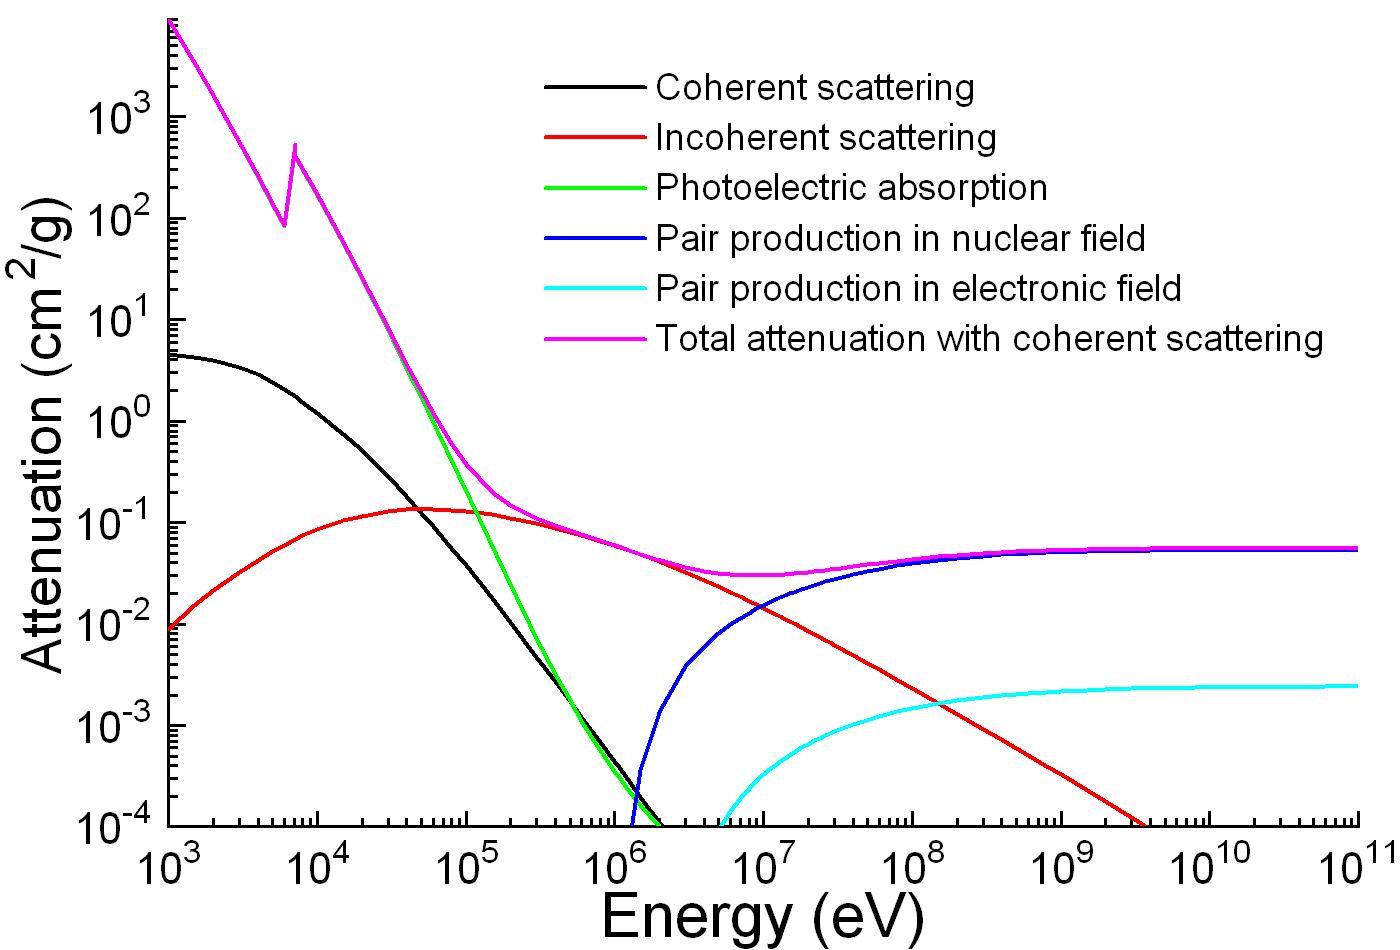
\includegraphics[width=0.7\linewidth]{../fig/intro/Ironattenuation}
	\caption[Mass attenuation coefficient of iron.]{Mass attenuation coefficient of iron. \footnotemark}
	\label{fig:attenuation_iron}
\end{figure}

\footnotetext{image source: by Materialscientist - \url{https://commons.wikimedia.org/wiki/File:Ironattenuation.PNG}, CC BY-SA 3.0 (\url{https://creativecommons.org/licenses/by-sa/3.0}) or GFDL (\url{http://www.gnu.org/copyleft/fdl.html}), via Wikimedia Commons}

\section{Basics of Radiobiology}
\label{sec:cell}
\subsection{The human cell}
All higher organisms consist of cells working together to form what is called tissue.
A collection of tissues which perform one or more functions is considered an organ. \\

Even though different types of cells exhibit distinctive traits which set them apart, all of them originated from the same totipotent zygote containing an original set of DNA.
A zygote is a stem cell, it has the ability to replicate indefinitely, passing its DNA on to the resulting daughter cells.
At the same time, it can change into any type of body cell. This feature is why it is called 'totipotent'.
As soon as the zygote has divided into a sufficient number of identical cells, all of them differentiate into the various human tissues.
In favour of becoming more specialised, cells lose their totipotency.
During the early stages of an embryo they are still capable of developing into a number of different cell types, but already restricted to their own tissue type; either nerve, skin, or blood \& muscle tissue.
As those cells further specialise, they limit their potential even more.
In a fully grown human body there are still stem cells present, such as bone marrow stem cells.
Other than the zygote, bone marrow can only give rise to blood cells, but not to e.g. nerve or skin cells.
A blood cell itself cannot replicate, it is considered a 'mature cell'.

The whole process follows guidelines dictated by the DNA.
Every cell inherited its own personal copy of the original set.
Inevitably, mistakes happen during its replication resulting in changes to the DNA called 'mutation'.
Most of these alterations are repaired or do not lead to changes in the cells behaviour.

The time needed for a reparation process to be completed is not the same as the period between cell reproduction. Changes to the DNA (e.g. mutations) occurring less frequently than one reparation cycle are less probable to result in permanent alterations, than those taking place more frequently. This is the reason why cells in tissues and organs that divide more frequently (i.e. gonads) are more prone to, for example, radiation induced mutations than those reproducing more slowly (i.e. bones).

As the human body ages, the repair mechanism loses some of its efficiency and mutations accumulate.
At one point, a cell may be reprogrammed to act in an unpredictable way, giving up its duties and duplicating without restraint, possibly forming tumours.
Also, external factors are known to influence cell behaviour and induce such 'malign' cells (carcinogenesis).
Cancer cells usually replicate more frequent than healthy cells, eventually leading to characteristic symptoms.

Different approaches have been developed to treat cancer, not all of which are suited to tackle every type of tumour.
If the tumour's location is unknown or metastases have formed already in many places, chemotherapy might be considered.
An easily accessible tumour could be removed in a surgery.
Non invasive therapies also include radiotherapy, destroying cancer cells using ionising radiation. (see chapter \ref{sec:irradiate}.)

Generally, early treatments have high chances of success, but tumours are often not noticed until they reached a certain stage. 
Reliable ways of diagnosing tumours are made possible by imaging techniques visualising the interior of the human body. \cite{Baumann2017, joiner2009}

\subsection{Effects of radiation}
\label{sec:irradiate}

Cell damage could either be caused by radiation interacting directly with the critical target in a cell or with other molecules and atoms within the cell.
For X-rays, two thirds of the biological damage is attributed to indirect action.
As described in \ref{sec:photon}, radiation transfers some of its energy to the medium it passes through.
Most interactions, such as the photo effect, incoherent (Compton) scattering and pair production, result in free electrons.
This is why it is called "ionising radiation".
If the electron has a sufficiently high kinetic energy, it may free additional orbital electrons from atoms in its vicinity.
The remaining ions are positively charged, with a single unpaired valence electron.
This type of chemical and free electrons are both referred to as 'radicals' and considered extremely reactive.
As the human body consists mainly of water, the radicals created are often $H_2O^+$ (water ion) and $OH \bullet$ (hydroxyl radical).
They are likely to take part in chains of chemical events leading to the breakage of chemical bonds which can disrupt the structure of macromolecules.
Such processes can induce changes in DNA sequences and eventually produce biological damage. \\

A irradiated cell can be affected in various ways ranging from no effect to immediate cell death.
The cell might also survive containing a minor mutation.
A more fundamental mutation might lead to carcinogenesis.
Irradiated cells might also send signals to their neighbours, inducing genetic damage known as 'bystander effects'.
On the other hand, surviving cells can also react to irradiation and becoming more resistant.

One classification separates cell damage into lethal, sublethal or potentially lethal.
Sublethal damage can be repaired, provided it occurs only once before the repair cycle is complete.
Potentially lethal damage can be manipulated by repair, provided the cell is allowed to remain in a non-dividing state.\\

The relative biological effectiveness (RBE), which describes the damage done by a specific type of radiation (compared to a reference test radiation) to a certain type of tissue, is dependent on various factors, including the rate at which dose is delivered.
In the case of radiation causing sublethal damage, for instance, the dose rate significantly affects the RBE.
If the average time between two sublethal damages in a single cell is longer than the time necessary for a full repair cycle, the cell will have a fair chance of survival.
Does it sustain damage more frequently, the cell will die with a much higher probability.
Increasing the radiation rate above this threshold results in a jump of the RBE.

Raising the RBE does not automatically correspond in better treatment.
Only if a differential effect reduces the RBE for healthy tissue compared to the tumour, there is a therapeutic advantage.
Fortunately, tissues react differently to the same type of radiation.
This behaviour can be used to increase the RBE for tumours and reduce it for healthy tissue.\\

On a larger scale, the sum of damages done to individual cells gives rise to characteristic symptoms.
Generally, these harmful effects of radiation are defined as either stochastic or deterministic.
The probability of stochastic effects is directly proportional to the dose, but their severity in affected individuals is not.
These effects arise in single cells (e.g. carcinogenesis), and it is assumed that the probability for such an occurrence is always greater than zero, even for small doses.
If many cells show mutations, the probability of cancer development is higher, but the symptoms of growing tumours will not be worse.
For deterministic effects, on the other hand, the severity scales with the dose.
They are connected to tissue reaction caused by damage to a population of cells.
The higher the dose, the more cells die, the graver are the biological consequences.

Changes to the DNA might not become apparent ever, others take years until they result in biological effects.
The same goes for tissue effects, which could either be acute (soon after exposure) or delayed (chronic).
A possible long term consequence of ionising radiation is leukaemia.
Damage to germ cells (sperm/egg) might even result in genetic damages expressed in subsequent generations.


While imaging modalities utilising X-rays are designed to apply a dose as little as possible to keep effects of irradiation low, radiotherapy makes use of the lethal effects targeting cancer cells. \cite{Podgorsak, Maidment2014}

\section{Imaging modalities}

The imaging of human body's interior has diametrically changed medicine.
It has its use in almost all medical disciplines.
Currently, there are many ways to acquire section images (or also volumes) of our organism without causing serious and sustained side effects.
They differ not only in size of the depicted volume and the image quality, but also in what additional information they provide besides purely morphologic data.
These other features can be functional, for example describing effectiveness of a metabolic process; or even molecular, revealing pathways of a certain molecule's distribution.
In the next chapters, X-ray planar imaging and the imaging modalities used for this thesis (computer tomography and magnetic resonance imaging) will be explained in more detail.


\subsection{X-ray projection imaging}
A widely used imaging technique based on photon interactions is X-ray projection.
Its setup is made up by a radiation source, the object of interest and a detector.
Since the technique is about projection, a patient needs to be placed between an X-ray tube and the detector (usually a film-cassette or digital sensor).
In the first stage of the imaging process, X-ray photons emitted by the tube enter the body.
Next, while travelling through human tissue, they interact with its atoms in various ways as described above (see \ref{sec:photon}).
These processes govern how much radiation is absorbed or scattered.
Finally, photons which make it through the patient are recorded as they reach the detector on the opposite side.
This results in a negative greyscale image, where brightness values correspond to the intensity reduction.
Low intensity (= high absorption) leads to bright spots on the image and vice-versa.
The whole process could also be described as 'the projection of attenuation shadows onto the detector', since the radiation absorption directly depends on the attenuation coefficient. The attenuation, on the other hand, depend on the tissue's properties (e.g. atomic number Z, density, etc).
Consequently, the attenuation shadows depict a projection of the patient.

\subsubsection{Soft tissue contrast}
\label{sec:soft}
Soft tissue such as brain matter and muscles absorb only little radiation, casting a lighter shadow (dark areas on image) than bone which absorbs more photons (bright areas).
Practically, in the human body, anything other than bone differs only slightly in attenuation, owing to the relatively small difference in atomic numbers and density.
For this reason, X-ray projection imaging is considered reliable when it comes to diagnose bone fractures, while at the same time, it is not suited to clearly delineate soft tissue structures.
The use of contrast agents, which effectively increase the density (atomic number) of certain structures or fluids, can help tackle this shortcoming.
Such substances fill e.g. the bloodstream with heavier atoms, which can be clearly seen against the dark background of surrounding soft-tissue.
In CT angiography, for instance, iodine is administered intravenously enhancing vessel to vessel-wall contrast.
In studies of the abdomen a diluted iodine solution or barium compounds swallowed by the patient leads to improved visibility of the gastrointestinal tract.
For some examinations, the patient inhales a contrast agent.

For patients allergic to those chemicals, a number of alternative agents have been developed.
Unfortunately, most introduce minor, sometimes serious side-effects.
There is ongoing research to find materials yielding enhanced contrast while at the same time minimising adverse reactions, a promising candidate being gold nano particles. \parencite{Podgorsak, Maidment2014}


Other imaging modalities are potentially better suited for soft tissue imaging, like medical ultrasound and Magnetic Resonance Imaging (MRI), to name a few.
They are preferred for non invasive soft tissue examinations.
The choice of suitable imaging modality depends a lot on the particular diagnostic needs and capabilities.
It is for the clinician to decide how detailed the information needs to be and how fast it has to be provided.
Often less accurate and/or cheaper methods are used first and, if necessary, followed by more sophisticated ones.


\subsection{Computer Tomography - CT}

Computer Tomography (CT) is a three-dimensional (3-D) imaging modality based on the measurement of X-ray planar projections.
The technique has evolved from 2-D X-ray scanning.
By mounting source and detector on a rotary ring with a patient at the centre, projections from any angle can be obtained.
However, in contrast to 2-D projection methods, the detector resembles an arc made up by several hundreds of neighbouring detector elements.
A single 'image' taken by the detector is therefore only in 1-D.
Yet, by repeating this process from a sufficient number of different angles and along the entire patient (z-axis) a 3-D model can be computed (based on 'Radon transformation').
In contrast to 2-D methods, where the patients interior is projected/compressed onto a flat image, CT preserves the exact location information. This feature led to a radical improvement in diagnostics.	 \\

Since its clinical introduction in 1971 by Godfrey Hounsfield, CT has become a widely used 3-D imaging modality for a range of applications including radiation oncology. Especially in radiation therapy, knowledge of the exact geometry is crucial, which is why CT plays such a pivotal role in treatment planning (see \ref{sec:planning}). \cite{Podgorsak, Maidment2014}

\subsubsection{3-D image reconstruction}
As a photon passes through the patient, it encounters different materials associated with characteristic linear attenuation coefficients.
It is practical to think of the scanned body as a collection of $N = N_X\cdot N_Y\cdot N_Z$ finite size cubes ($\Delta x$ cube length) called 'voxels' (analogous to pixels in a 2-D digital photograph).
The entire model can then be regarded as a 3-D matrix, with the attenuation coefficients $\mu_i$ of the voxels as its entries.
Figure \ref{fig:voxel_matrix} represents a ($4, 4, 1$) matrix.
It depicts the path an X-ray may follow passing through voxels with different values $\mu_i$.
This discretisation allows us to change equation \ref{eq:mu_int} to:
\begin{align}
\label{eq:mu_sum}
I(x) = I_0 e^{- \sum\limits_{i=1}^{N_X} \mu_i \Delta x}
\end{align}

The initial and final intensities can be read of the settings of the X-ray tube and the detected signal.
Based on these values, image reconstruction algorithms derive the three-dimensional linear attenuation coefficient matrix.
For convenience, the computed numbers are converted to Hounsfield Units which are displayed in the final image. \cite{Podgorsak, Maidment2014}

\begin{figure}[!htb]
	\centering
	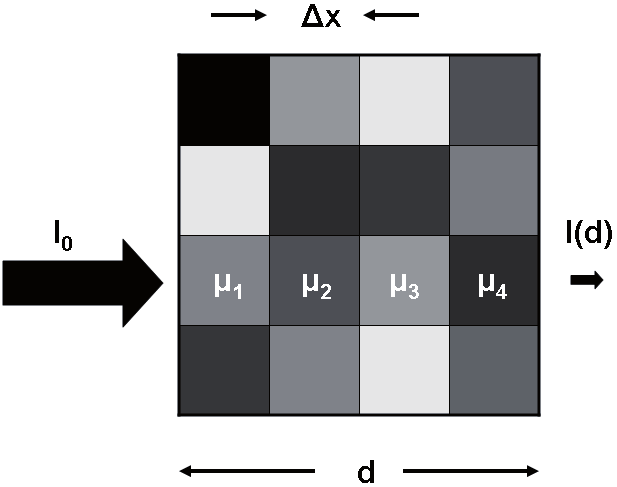
\includegraphics[width=0.5\linewidth]{intro/screenshot001.png}
	\caption{Simplified attenuation matrix (4,4,1). Image source: \cite{Maidment2014}}
	\label{fig:voxel_matrix}
\end{figure}

\subsubsection{Hounsfield Units}

In a final CT scan, voxel values are recorded in Hounsfield Units (HU), which relate to the attenuation of water at room temperature:
\begin{align}
HU_{material} = \frac{\mu_{material} - \mu_{water}}{\mu_{water}} \cdot 1000
\end{align}

Table \ref{tab:HU} lists types of human tissue and their values on the HU scale.
Generally, HU values range from -1024 to +3071 (12 bit), but the upper limit can be extended to 15,359 (14 bit) if materials with even higher attenuation need to be visualised (e.g. implants). \\

\begin{table}[]
	\centering
	\caption{Average HU values for various types of human tissue.}
	\label{tab:HU}
	\begin{tabular}{@{}ll@{}}
		Substance           & HU                     \\
		\toprule
		Air                 & –1000                  \\
		Lung                & –750 (–950 to –600)    \\
		Fat                 & –90 (–100 to –80)      \\
		Water               & 0                      \\
		Muscle              & +25 (+10 to +40)       \\
		Brain, white matter & +25 (+20 to +30)       \\
		Kidneys             & +30 (+20 to +40)       \\
		Brain, grey matter  & +35 (+30 to +40)       \\
		Blood               & +55 (+50 to +60)       \\
		Liver               & +60 (+50 to +70)       \\
		Compact bone        & +1000 (+300 to +2500)
	\end{tabular}
\end{table}

Typically, CT scans are displayed on computer monitors, which imposes the need to map the HU values to a 8-bit greyscale (256 steps of luminosity).
Since the number of possible values (dynamic range) on the HU scale is 16 times the shades of grey on a screen (12-8 = 4 bit difference; equivalent to a factor of $2^4$) the screen cannot convey all details at the same time.
A linear mapping would result in 16 neighbouring HU values being compressed to the same brightness on the screen.
This way, the brightest (bone) and darkest parts (soft tissue) of the image would be clearly distinguishable.
At the same time small differences (<16 HU) would appear to have exactly the same intensity.
However, most of the time, the doctor's focus might lie either on soft tissue or bone material.
Bearing in mind that soft tissue values range only from 10 HU to 70 HU at most (see table \ref{tab:HU}), such a compression would make distinguishing tissues using CT very unreliable.
Instead of showing detail from the lowest to the highest value, a range of values - a so called window - can be chosen.
Let's assume, for example, a range from -100 to 155 HU to be of interest.
This selected range can be mapped directly and uncompressed to a 8-bit greyscale.
Any values above 155 HU will be assigned the brightest value (white = 255), below -100 the darkest (black = 0).
While showing very good soft tissue contrast, all bones would be depicted with exactly the same brightness (255), even though they might have a varying HU values.
For bone structures, a range from 300 to 2500 HU might show sufficient contrast.
Standard computer programs used to display CT images allow the user to change the window interactively to any value range. \cite{Podgorsak, Maidment2014}

\subsubsection{Image acquisition}
The time necessary to collect 1-D attenuation projections from sufficient angles is called 'acquisition time'.
In 2-D X-ray scanning only one picture is taken, while a 3-D CT model is made up of a photo sequence.
If the patient moves during the imaging process, the final model would show motion artefacts which might lead to wrong conclusions.
Consequently, CT scanners are designed to minimise acquisition time while ensuring sufficient image quality.
Very fast CT protocols result in smaller resolution, because less images are taken.
It has to be said, though, that CT acquisition time is usually already significantly shorter than MRI. \cite{Podgorsak, Maidment2014}

\subsubsection{Image quality} %282
Additionally to the relatively short acquisition time, CT scans show little distortion compared MRI (see \ref{sec:MRI}), which is why they are often used as 'gold standards' (reference scans used for MRI distortion assessment).

While bone structures are clearly visible in CT scans, 'soft tissue contrast' is relatively low compared to MRI.
In other words, parts of the body which are considered as 'soft tissue' (intestines, brain, blood vessels, etc.) differ little in brightness and are therefore hard to distinguish.
See \ref{sec:soft} for more information.

Another aspect of image quality is the 'low contrast resolution' of the scan.
It directly relates to how much structures and their surroundings have to differ in signal intensity to be clearly distinguishable by doctors.
The quality of the 'low contrast resolution' is mainly limited by noise.
Noise is a random pattern underlying the actual signal and is always present to some extent.
Its prominence in the final image is described by the Signal to Noise Ratio (SNR).
If the SNR is too low, fine structures blend with the noise and cannot be distinguished. 
Strategies to achieve a high SNR include raising the initial photon flux (intensity) or employing contrast agents.
The intensity is governed by the tube current, which is limited by the heat capacity of the tube and health considerations regarding the patient dose.

Alternatively, the spatial resolution can be decreased, effectively combining neighbouring image slices.
This way the SNR for the combined slices is increased, but fine structures along the z-axis might be lost due to the reduced resolution. \cite{Podgorsak, Maidment2014}

\subsubsection{Health considerations}
CT scans describe the attenuation throughout a patient, which is directly related to how much energy is transferred from photons to matter.
Only because X-rays are absorbed by the human body, this imaging modality gives insight in the density distribution of a body's interior.
However, this transferred energy is capable of causing biological damage. (see \ref{sec:irradiate})

While the radiation dose administered during a single CT scan is relatively small (typically not more than 15 mSv) and almost negligible compared to the dose administered during a potential radiation therapy, patients receiving this dose regularly end up with a potentially harmful accumulated amount of radiation.
Cancer patients, for instance, need to be imaged frequently during treatment planning.
However, patients might die before those consequences come into effect.
Therefore, it is typically children (who received a great number of CT scans) to suffer from induced cancer occurring up to 40 years later.
So while the benefit from using CT for diagnostics far outweighs the damage, there have been major efforts to reduce dose while maintaining reasonable image quality.
\cite{Sodickson2009, McCollough2009, Murphy2007, Smith2007, Goldman2013, Brenner2001}


\subsection{Magnetic Resonance Imaging - MRI}
\label{sec:MRI}
Magnetic Resonance Imaging (MRI) is a 3-D imaging modality based on Nuclear Magnetic Resonance (NMR), a phenomenon discovered by physicist Isidor I. Rabi in 1938.
Atomic particles such as protons have an inherent quantum mechanic feature called 'spin', which is associated with a magnetic moment $\mu$.
Without an external field, a proton's spin is oriented in a random direction in space and so is its magnetic moment.
The sum of magnetic moments belonging to a number of protons results in a net magnetisation.
Due to their random orientation, the net magnetisation will be zero for a sufficiently high number of particles.
This is because, on average, for every proton's spin there is always another particle's spin oriented exactly the opposite way cancelling its magnetic moment.

In the case of an applied external magnetic field (this static field is often called $B_0$), the spins will either align parallel (pointing in the same direction) or anti-parallel (opposite direction) to this field, where their energy reaches a local minimum.
Parallel protons have an even lower energy than those pointing the other way.
In a collection of many spins, the number of parallel spins will therefore slightly dominate, resulting in a net magnetisation greater than zero (see figure \ref{fig:spin_align}).
In other words, only the amount of protons that is not compensated by those looking in the opposite direction contributes to a detectable magnetic field.

\begin{figure}[h!]
\centering
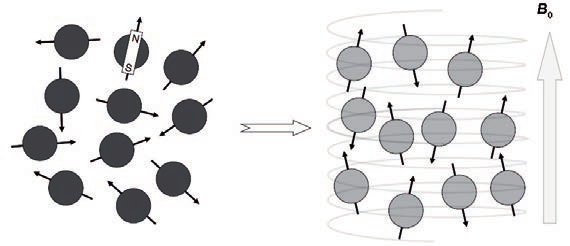
\includegraphics[width=0.8\linewidth]{../fig/intro/spin_align}
\caption[The spins, initially oriented randomly, become aligned either parallel or antiparallel to an extern magnetic field $B_0$. Image source: \cite{Maidment2014}]{The spins, initially oriented randomly in space, become aligned either parallel or antiparallel to an externally applied magnetic field $B_0$. Image source: \cite{Maidment2014}}
\label{fig:spin_align}
\end{figure}

By applying a short radio frequency pulse (often referred to as $B_1$), the total external magnetic field changes and the magnetic moments start precessing around that new external field.
The pulse duration is usually chosen as to flip the spins by a $90^o$ angle.
They are now oriented in the transverse plane to the original external field, and so is the resulting net magnetisation.
Similar to how a spinning top rotating at an angle to the direction of gravity precesses, the magnetic moments will now precess about the direction of the external field with a frequency linearly proportional to the external field strength.
This precession movement can be detected as induced current in a receiver coil, because the net magnetisation still follows the spins' orientation. 
Again, the particles would like to minimise their energy by aligning their spins to the external field, but in order to do so they need to give away the surplus energy, transferring it to the surrounding lattice.
Those spin-lattice interactions happen with different efficiency depending on the tissue.
The time it takes the spins to align is expressed in a material specific time constant $T_1$.
Shortly after applying the radio frequency pulse, regions of the body where magnetic moments align quickly (short $T_1$) have a stronger net magnetisation (in the direction of the external field) than those where energy is being transferred slowly (long $T_1$).

At the same time, the spins interact with each other, affecting the local magnetic field and spins in their vicinity.
The magnetic moments, which started out precessing in phase directly after the radio frequency pulse flipped them, will precess at slightly different frequencies, due to the small fluctuations of the local magnetic field.
The differences cause the collection of magnetic moments to 'de-phase' and the net magnetisation in the transverse plane to vanish.
This process caused by spin-spin interactions is described by the material specific time constant $T_2$.
Eventually, all spins will be again aligned either parallel or anti-parallel to the external field, just as they were before the RF-pulse.

Applying the RF pulse with a homogeneous field strength along the whole body would excite all spins simultaneously.
In order to localise differences in tissue magnetisation, the RF pulse is instead combined with a linear magnetic gradient field 'selecting' a slice to be imaged at a time.
The rest of the body is unaffected, the signal measured directly after such a pulse was applied originates only from the chosen slice.
Eventually, by collecting data on the net magnetisation throughout the body in different locations ('scanning' the patient slice by slice), a 3-D image can be computed.

Depending on the information required from the examination, Doctors can choose to create images that reflect spin-lattice interactions ($T_1$ weighted) or spin-spin interactions ($T_2$ weighted).

Governed by the chosen settings, particular tissues will displayed varying contrasts.
For example, areas with increased water level will be dark on T1 weighted ($T_1w$) MRI whereas the same areas will be bright on $T_2w$ MRI.
Additionally, certain types of materials (tissues) can be intentionally not imaged (suppressed) to reveal others that are in their close proximity.
This is often done with fatty tissue that can cover relevant parts of the field of view.
There are various methods how this can be achieved.
MR imaging gives practically endless possibilities in terms of selective imaging and is mostly limited to imaging time and technical characteristics of the scanner.
Medical physicists and scanner vendors are incessantly working on new MR imaging methods and applications. 

The set of parameters governing how the tissue is excited and data acquired is called 'image sequence'.
Delineating tumours or lesions is often accomplished by looking at both $T_1w$ and $T_2w$ weighted images and drawing the right conclusions.

Soft tissue contains a lot of water, which is made up by oxygen and hydrogen.
Hydrogen nuclei are single protons and their nuclear magnetic resonance is what MRI is tuned to visualise.
This is why soft tissue appears as bright areas in MRI, whereas bone material has only little contrast. \cite{Currie2013}


Most the scanners are build to house a receiver coil in the gantry and they are able to measure the signal using only this one coil.
However, in practise, to obtain a stronger signal, a smaller coil is typically placed closer to the source of the signal, the patient.
As the region of interest (ROI) is usually limited to a specific organ, receiver coils are available in different sizes and shapes, often designed to fit the patient with a comfortable but narrow space in between.


To get even closer, so called 'surface coils' can be placed on the patient.
'Spine coils' are sometimes hidden in the table on which the patient lies during the examination.
Typically, for creating images of a patient's head, coils with a fixed arc-like geometry are used.
This type of coil (see figure \ref{fig:coil}) was used for the data acquisition of this thesis.

\begin{figure}[tbh!]
\centering
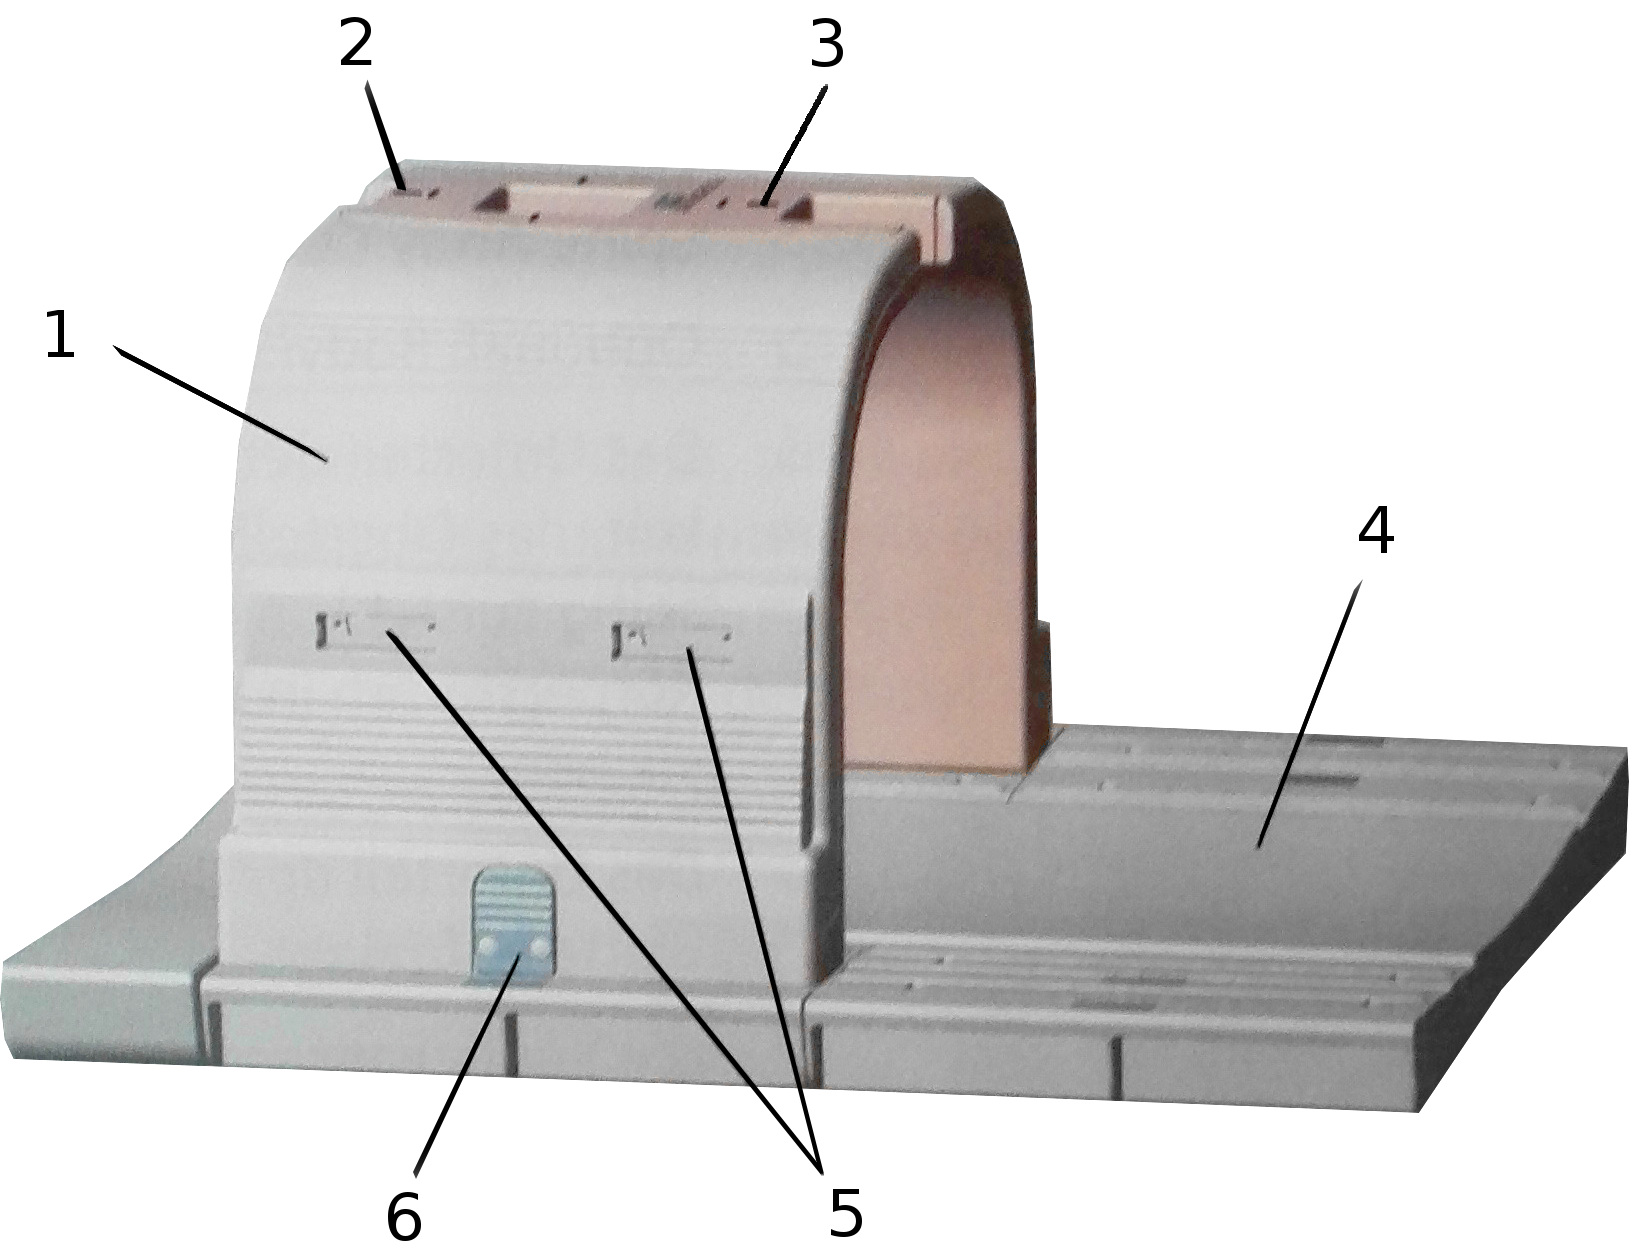
\includegraphics[width=0.6\linewidth]{scanner/coil}
\caption[MR scanner coil. Image source: Siemens Healthineers]{MR scanner coil: (1) upper part, Body/Spine Array Coil; (2,3) central positioning markers; (4) lower part, Body/Spine Array Coil; (5) connection ports; (6) colour label. Image source: Siemens Healthineers}
\label{fig:coil}
\end{figure}

Studies have shown that delineating certain types of tumours, for example prostate cancer, is more accurate using MR images than using CT. \cite{Rasch1999, Debois1999, Roach1996}

In diagnostics, MR images prove to be very useful.
Also for radiation therapy treatment planning, the superior soft tissue contrast is exploited during the definition of organs at risk and targets.
Unfortunately, due to the physical principles of MRI, it indirectly provides the information about the proton density, whereas CT can provide information about electron density.
It is the knowledge of the electron density which is necessary in the treatment planning process.
During this, the dose distributions are calculated based on the applied beam geometry and the distribution of matter on its way.


\subsubsection{Image Quality}
Contrary to CT, MRI is prone to distortion due to field inhomogeneities.
Organs might appear shifted, elongated or shrunk.
The effect is most prominent along the outer edges of the scanner's field-of-view (FOV).
In the isocentre (middle) of the scanner, the distortion is smaller, because here the field is least aberrant.
For most applications, small position shifts and deformations are of minor importance.
MR scanners usually come equipped with an internal distortion correction algorithm.
Figure \ref{fig:dist_compare} shows the unmodified and the corrected version of an image coming from such a scanner.
Those methods are developed by the company designing the scanners.
Knowing the technical details enables them to write tailor-fit scripts which drastically reduce the distortion.

However, for radiotherapy treatment planning this might not be enough and it is necessary to additionally monitor the distortion and, if necessary, take additional corrective measures. 

While its soft tissue contrast is superior to CT, a relatively long acquisition time is necessary to achieve a sufficiently high SNR.
This leads to the risk of motion artefacts (patients moving during the scanning procedure).
To tackle this issue, resolution can be reduced, effectively combining signal from several voxels to create a single voxel, reducing the overall noise.
The trade-off is that fine structures might get lost.

\begin{figure}[h!]
\centering
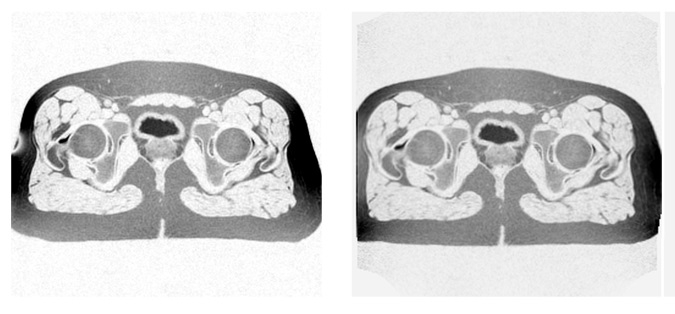
\includegraphics[width=\linewidth]{../fig/vgl-corr_inverse.jpg}
\caption[MR image before and after applying build-in distortion correction. Image source: Courtesy Piotr Andrzejewski (unpublished data)]{On the left is the original image, on the right the automatically corrected version of the same MR image (inverted colours). Image source: Courtesy Piotr Andrzejewski (unpublished data)}
\label{fig:dist_compare}
\end{figure}

%Field of view (FOV) of the MR scanner is smaller than the CT scanner's.


\subsubsection{Health considerations}

Strong, static magnetic fields (typically up to $3\, T$) are present around MR scanners at all times, and precautions have to be taken to ensure safety for patients and medical personnel.
Ferromagnetic materials (such as steel and iron) can become dangerous projectiles in vicinity of the MR scanner.
They must be excluded from the room housing the magnet without exception.\\

%It is also important to remember that medical implants, including but not restricted to cardiac pacemakers and hearing-aids, might malfunction or become damaged in strong fields regardless whether they contain ferromagnetic materials.
%Patients with such implants might still be imaged with scanners utilising weak fields up to $0.5\, T$.

The RF pulses repeatedly put spins in excited states, transferring energy to the human body.
MR scanners are designed to limit the rise of a patient's body temperature to $0.5\,^o$C during standard imaging.
Only combined with either medical or appropriate psychological monitoring the limit can be raised to $1\,^o$C.
An ethics committee approval is necessary for even higher values.
In general, patients should be exposed to RF fields only as strong as their thermoregulatory system is capable to cope with.\\

Finally, magnetic field gradients are applied together with the RF pulse.
They are switched at high frequencies leading to induced currents in conducting body tissue.
In principle, those currents stimulate nerves which might result in muscle twitching or pain.
However, gradient levels are set to avoid stimulation.
During have reported some subtle biological effects, but there was no evidence pointing towards harm caused by short term exposures.
At the same time, patients suffering from epilepsy might show increased sensibility to induced electric fields in the cortex and should be imaged with caution. \cite{Maidment2014}
Some patients might be allergic to contrast agents used for specific MRI examinations.
Here, safety procedures are similar to those performed during administration of regular drugs. 

\subsubsection{Open bore MR scanners}

The radiation oncology department of the Vienna General Hospital (AKH) is equipped with a $0.35\, T$ open-bore, c-arm MR scanner (see Section \ref{sec:magnetom} for more details).
This open design has proven to drastically improve the well-being of patients experiencing anxiety in closed-bore scanners.
For this reason, the number of incomplete MR examinations due to a claustrophobic events is relatively low. \cite{Enders2011, Bangard2007}
Besides, patients who would not fit in closed designed scanners can be imaged.
Furthermore, brachytherapy patients can be placed in the scanner with applicators attached.
Brachytherapy is a form of radiation therapy in which radiation sources are typically inserted into the human body to perform the irradiation from close distance; imaging is performed for dose distribution planning as well as verification of applicators position after their insertion (for more information see section \ref{sec:planning}).

This scanner's magnetic field is weaker than the fields of closed-bore scanners that are widely used (typically 1-3 Tesla).
High field strengths result in greater resolution, better SNR ratio and faster imaging time.
Generally, diagnostics benefit from greater image quality.
However, at some point, diagnostic accuracy stops increasing with field strength.
At the same time significant improvements can be achieved at low fields.
A ``combination of field independent polarisation [...] with frequency optimized MRI detection coils [...] results in low-field MRI sensitivity approaching and even rivalling that of high-field MRI.'' \cite{Coffey2013}

Low field MR scanners are also typically characterised by less distorted images. \cite{Fransson2001}

Apart from the often satisfactory image quality, there are considerable cost advantages to the use of lower field MRI.
The initial purchase price and the ongoing maintenance expenses are considerably lower than those of high field scanners, which often use superconducting magnets cooled with liquid helium. \cite{Rutt1996}
Permanent magnets might be weaker, but do not require constant cooling.
Also, low fields allow facilities to build smaller rooms and magnetic objects are less dangerous.


\subsubsection{Diffusion Weighed Imaging - an example for non morphologic Imaging}

Despite the fact that this type of MR imaging was not used for this thesis, it will be mentioned here as an example of the vast range of measurements possible with MRI techniques.\\

% https://www.youtube.com/watch?v=J_aamnpRJE8
% MRI - from picture to proton S. 331 (im pdf auf 344)
Diffusion weighted (DW) imaging quantifies molecular diffusion in the body.
This imaging technique uses MRI technology differently:
Additionally to the gradients needed to select a slice (strength $~3-5\, mT/m$, duration $2-4\, ms$), the sequence for DW imaging applies two long, strong, consecutive and opposite gradients (strength $~30-50\, mT/m$, duration $20\, ms$) during which molecules may move due to diffusion.
After those two gradients (which, usually, will be applied in all three Cartesian directions), the remaining signal (net magnetisation) is measured by the receiver coil.

Molecules which are restricted in their movement will experience two equally strong but opposite magnetic fields.
The first will cause them to precess with a certain speed (linear with field strength), effectively changing their phase.
The second will cause them to precess exactly the other way around (same strength, but other direction), returning them to their initial state.
Now they will again be in phase and result in a net magnetisation which is not zero, but visible as bright areas on the scan.

Those molecules which are free to move, however, will not experience a constant field strength, because the field has a gradient.
As they move through the body they will precess at varying speeds during the first and then at different speeds during the second gradient.
As a result, they will be out of phase when the net magnetisation is measured by the receiver coil, and will not cause bright areas in the scan.

DW imaging can be used to diagnose acute strokes (brain infarct), because areas with restricted diffusion (blocked blood flow) show a strong signal compared to healthy tissue with normal diffusion.
Another interpretation of low diffusion (high measured signal) can be the increased cellular density (so dense that free diffusion of water molecules is suppressed) which is characteristic for cancerous tissue.\\

Since the time necessary to allow the molecules to move during the two gradients is relatively long, the image will naturally be $T_2$ weighted.
This is taken into account by creating a second image which is also $T_2$ weighted, but does not apply two consecutive opposite gradients.
The difference between the DW and the not DW weighted sequences reflects the actual contribution of diffusion (apparent diffusion coefficient - ADC). \cite{McRobbie2006}


\section{Radiation therapy}
\label{sec:planning}
Radiation therapy utilizes ionising radiation to damage or kill cancer cells in order to stop them from multiplying.
This prevents the growth of tumours, makes them shrink in size and hopefully cures the patient. 

During radiotherapy treatment planning (RTP), 3-D models of the patient are used to define targets (regions where the dose should be delivered to) and organs at risk (where the dose should be delivered to).
This ensures that vulnerable organs are spared from radiation while making sure the tumours receive sufficient dose.
Moreover, methods to quantify the amount of radiation that different body parts absorbed are needed, because the actual treatment might differ from the plan.\\

While travelling through matter most types of radiation release energy mainly due to coulomb interactions with the outer shell electrons of atoms.
Knowing the electron density of the targeted tissue area is therefore essential.
In order to reach a specific penetration depth, the particles' initial energy has to be chosen accordingly.
The necessity to treat the tumour with a required amount of radiation leads to a radiation therapy treatment plan.

There are two well established methods for applying the radiation.
External beam radiotherapy (EBRT) is performed from afar:
Gantries are able to position the radiation source around the patient in a way covering virtually any possible angle.
During a treatment session, fractions of the total dose are administered from many different angles (or continuously with alternating gantry angle).
The sum of those individual treatments results in the required dose distribution.
Figure \ref{fig:plan} shows an example of two differently calculated treatment plans.

In conventional EBRT, photons (X-rays) in the range of $4\, MeV$ to $20\, MeV$ are used to deposit the necessary dose at the location of the tumour.
Unfortunately, radiation interacts with all cells it passes until it is fully absorbed.
It releases its energy along its entire path while travelling through the patient.
This behaviour may result in dose being delivered to cells all the way from the point of entry to the point where the (weakened) ray leaves the patient.
Other types of ionising radiation are also used, but less common.
Electrons and low energy X-rays are favoured for superficial tumours; rare methods using neutrons and even muons also exist.
Charged particle therapy (using e.g. protons or carbon ions) is on the rise, but far from reaching the availability of X-rays.
This type of radiation minimises the damage done to healthy tissue due to its distinctive behaviour in energy loss called ``Bragg Peak''.
They release most of their energy only shortly before being stopped completely.
\cite{Nakamura2010} This effect can be used to spare tissue lying behind the tumour from radiation entirely and also reduce the amount of energy transferred to organs located before. \cite{Paganetti2005}
A comparison between the behaviour of X-rays and protons is shown in figure \ref{fig:bragg}.\\

Brachytherapy, on the other hand, is when the radiation source is placed close to or inside of the patient.
The source is either moved close to the target area using applicators (temporary treatment) or implanted permanently.
The latter method is done by inserting so called "seeds" (sealed metal containers with radioactive material) directly into the target area where they release high amounts of radiation.
Over time they become less active and eventually the treatment stops automatically.
These rice grain sized implants can remain in the body without causing any harm.
Treatment of prostate and cervix cancer is often done with this technique.
In comparison to EBRT, Brachytherapy allows higher doses while at the same time minimising the radiation reaching organs at risk; precise dose distributions can be achieved.
At the same time, not all cancer types can be treated this way.
For some, a non-invasive method (e.g. EBRT) is a better alternative.\\


\begin{figure}[!tbh]
	\centering
	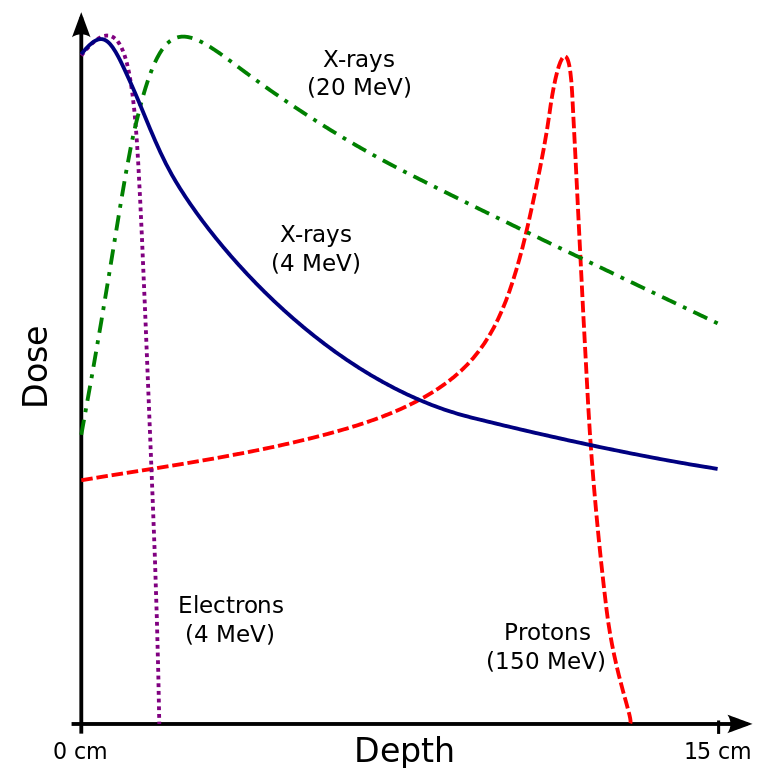
\includegraphics[width=0.6\textwidth]{Dose_Depth_Curves.png}
	\caption[Energy release of ionising radiation]{Energy release of ionising radiation \footnotemark}
	\label{fig:bragg}
\end{figure}

\begin{figure}[!tbh]
	\centering
	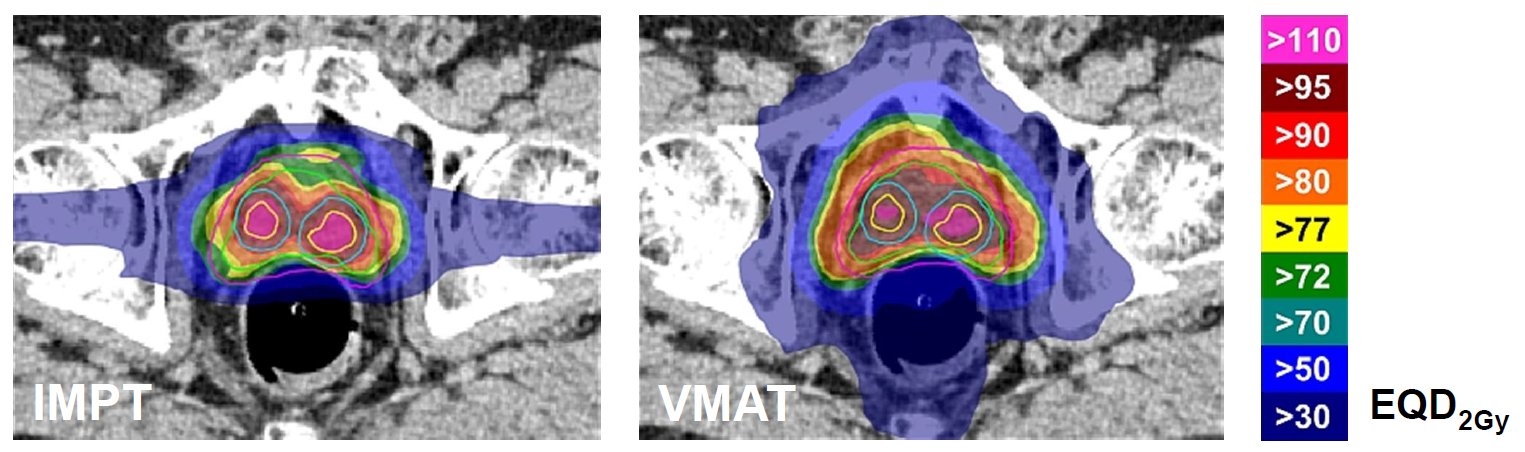
\includegraphics[width=\textwidth]{Plans.png}
	\caption[Example of Radiotherapy treatment plan (image source: \cite{Andrzejewski2015})]{Example of Radiotherapy treatment plan: coloured areas represent dose values deposited during treatment. The plans were calculated using different treatment techniques: with protons (IMPR) and photons (VMAT). Image source: \cite{Andrzejewski2015}}
	\label{fig:plan}
\end{figure}


\footnotetext{image source: by Cepheiden - \url{https://commons.wikimedia.org/wiki/File:Dose_Depth_Curves.svg}, [GFDL (\url{http://www.gnu.org/copyleft/fdl.html})], via Wikimedia Commons}

%\subsection{Types of radiation therapy}
%\todo{(Based on the IAEA Handbook Radiation Oncology Physics) Tele – is typically delivered in the range of few to some 20MV with linear accelerators (describe briefly the dose depth curve and that to be able to accumulate dose in the target and spare the OAR normally multiple number of beams is combined), typically photons are used but also electrons can be produced to treat superficial targets. For the latter also a low energy X-rays can be utilized – orthovoltage units. Then there are also havier particles to utilize like protons, neutrons or light ions – here few words about the Bragg peak. }


\subsection{Role of CT}

Until recently, RTP relied almost entirely on CT.
There are two main reasons for this:

Firstly, calculating the electron density using data obtained with CT is a straightforward task.
Secondly, CT images generate 3D images with little distortion. Exact geometries are needed for correct RTP.
It is the most reliable approach to create precise radiotherapy treatment plans. \cite{Constantinou2012, Schneider1996}

\subsection{Role of MRI}
MR images also record luminosity values, but they do not correspond to radiodensity.
Due to the better visibility of tumours on MR images, RTP often uses combined data from both imaging modalities.
Additional information derived from DW MRI, for instance, can also support response prediction and assessment.
However, there are some difficulties arising from combining CT and MRI for EBRT:
in order to profit from separately acquired data, the resulting images must be aligned (registered) either manually or automatically.
This is a hard task since non-rigid objects (organs) change their shape and location between measurements which may lead to inaccuracies.
Algorithms supporting non-rigid registrations are already under development, but there is still room for improvement.
For now, only local rigid registration is capable of reliable target and organ at risk definition.

Alternatively, MRI-only radiation therapy protocols are being developed:
one way of doing this is to use MRI data to create a Pseudo-CT, which contains information about electron density.
Comparisons of using CT and MRI-based pseudo CT have shown acceptable deviations for X-ray therapy.
In charged particle therapy the resulting dose gain in healthy tissue and dose loss in cancer regions owed to inaccurately assigned electron density values is bigger.
However, further improvement of accuracy promises to reduce time and money needed for RTP when CT is no longer needed.
Furthermore, patients would be spared the additional dose of CT examinations.  \cite{Rank2013, Stanescu2006, Jonsson2010, Greer2015, Chen2004}


\section{Aim of this work}
The idea of only using MRI for treatment planning is approaching the clinics, but there are still some issues that need to be addressed.

Due to the possible image distortion, great care needs to be taken and the MR images must be verified before they are used for RT target definition and dose calculation.
The available MR scanner at the AKH is equipped with an on board correction algorithm which is supposed to reduce distortion.
See figure \ref{fig:rendered_dist} for an example of how this correction affects an image.
Distorted images might lead to wrong calculations of how much energy is needed for the radiation to accumulate exactly at the target region.
If, for example, bone structure is depicted as thicker than it really is, RTP would suggest a treatment which would deposit more energy behind the tumour than intended.
The opposite holds for cases where tissue appears to be thinner, which would result in areas lying before the tumour being irradiated.

The goal of this work is to:
find an optimal (providing satisfactory image quality and convenience of use) liquid filling for the rod cavities in an already existing custom designed distortion phantom provided by the Medical University of Vienna to be able to acquire the reference CT image and test MR acquisitions.

Develop and implement a method to assess and illustrate the distortion of the MR image based on tracking of the distortion of one of the phantom rods, with an option to further extend the tool for multi rod tracking.

Therefore, this work focuses mainly on the assessment of the acquired imaging data (using the implemented software tools), choosing which liquids to fill the phantom with, but not its entire design.
However, possible fillings have to be produced and tested.
Similar approaches are being used for distortion correction by other facilities. \cite{Price2015, Petersch2004, Torfeh2015, Wang2004, Wang2004a, Mizowaki2000}


\begin{figure}[!thb]
\centering
  \begin{subfigure}[b]{0.49\textwidth}
  \centering
    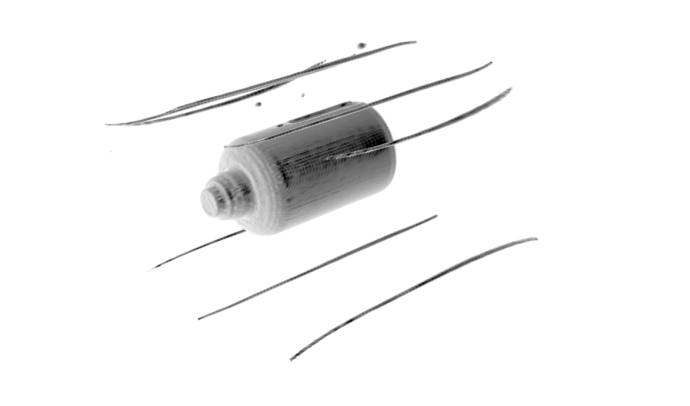
\includegraphics[scale=1.2]{rendered/rendered_MR.png}
    \caption{MR scan with no distortion correction}
    \label{fig:rendered_MR}
  \end{subfigure}
  \begin{subfigure}[b]{0.49\textwidth}
  \centering
      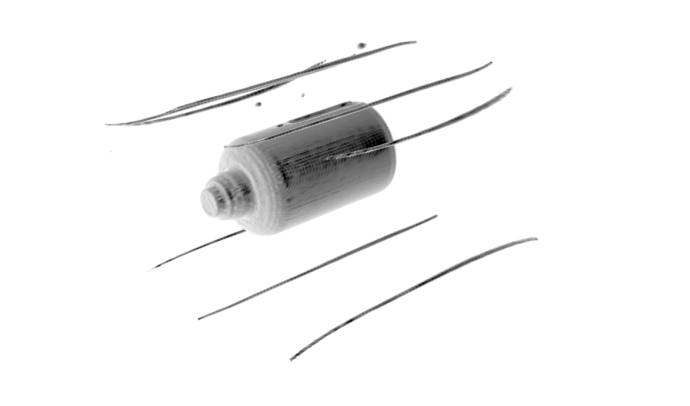
\includegraphics[scale=1.2]{rendered/rendered_MR_corr.png}
    \caption{MR scan after internal distortion correction}
    \label{fig:rendered_MR_corr}
  \end{subfigure}
  \caption[Rendered MR image before and after applying build-in distortion correction. Image source: Courtesy Piotr Andrzejewski (unpublished data)]{Rendered MR scan showing the difference before (a) and after (b) applying the build-in distortion correction Image source: Courtesy Piotr Andrzejewski (unpublished data)}
  \label{fig:rendered_dist}
\end{figure}


%to me \footnote{Auszug aus \citetitle{BohemRhap}~\cite{BohemRhap} von \citeauthor{Queen}~\cite{Queen} }\\
%\section{Farrokh Bulsara aka. Freddie Mercury}
%Weitere Zitate sind in Anhang \ref{appendix:zitate} zu finden.


\chapter{Material and methods}

%  Everything that is mentioned in results, has to be mentioned here
%  Everybody who reads thesis, must be able to reproduce the experiment/study
% o Describe all materials, devices and methods, which were used in your work
% o if you describe a device, start with the brand name followed by the company name, city and country in parentheses: e.g. "... a VersaHD (Elekta AB, Stockholm, Sweden) was used in ...".
% o Provide some information on each device
%  e.g Linac, which energies were used, what was the field size, what was the leaf width, how is the linac calibrated, ...;
%  e.g. Detector array: which type of detector, how many detectors, what is the resolution, energy dependence, linearity,...;
%  e.g. Panning systems: software version, algorithms, settings used in this study
%  e.g. software: version, functionality
% o Also describe used data (patient cohort) even if they were taken from other studies

\section{Scanners}

The radiation oncology department of the Vienna General Hospital (AKH) owns a open-bore, c-arm MRI scanner and a CT scanner (used as reference).
They are listed in Table \ref{tab:scanners}.

\begin{table}[h]
\centering
\begin{tabular}{llll}
System	& product name	& company	& coil [internal W x H]		\\
\toprule
MRI	& Magnetom C!	& Siemens	& Body/Spine Array Coil XL	\\
	&		&		& [50 x 30.5 cm (19.7 x 12 in)]	\\
CT	&		&		& --------
\end{tabular}
\caption{used scanners}
\label{tab:scanners}
\end{table}

\section{Custom build phantom}

To compare images from different scanners and asses occurring distortion, a rigid object with known dimensions is necessary.
Such a 'phantom' is often made from plastics containing a liquid.
The AKH's design is made up from an array of replaceable, fillable plastic rods.


\begin{figure}[!htb]
\centering
  \begin{subfigure}[b]{0.1\textwidth}
    
\includegraphics[scale=1]{slicer3D/full_phantom/sagittal_comparison_mr.png}
    \caption{MR}
    \label{fig:sagittal_comparison_mr}
  \end{subfigure}
  \begin{subfigure}[b]{0.1\textwidth}
    
\includegraphics[scale=1]{slicer3D/full_phantom/sagittal_comparison_ct_empty.png}
    \caption{CT}
    \label{fig:sagittal_comparison_ct_empty}
  \end{subfigure}
  \begin{subfigure}[b]{0.1\textwidth}
    
\includegraphics[scale=1]{slicer3D/full_phantom/sagittal_comparison_ct.png}
    \caption{CT}
    \label{fig:sagittal_comparison_ct}
  \end{subfigure}
  \caption{Comparison: MRI only shows liquid filling, CT also the plastic rod and pane (horizontal black bar crossing middle and right rod);\\ (\textbf{a:}) \textit{MRI} - filled rod, plastic not visible (field of view too small to show entire rod); (\textbf{b:}) \textit{CT} - empty rod, plastic visible; (\textbf{c:}) \textit{CT} - filled rod, plastic and filling visible}
  \label{fig:sagittal_comparison}
\end{figure}

\subsection{Frame and rods}

The phantom was build to fit the largest available rigid coil for the MRI scanner.
Three parallel acrylic glass panes in the shape of the coil serve as a frame for the plastic rods.
In the middle an empty area was reserved for an optional additional smaller phantom (not used for this work).
Figure \ref{fig:phantom_photo} shows a picture of the phantom. See also figure \ref{fig:axial_CT_pane} showing a CT image of one pane (with no rods inserted). \\
More than 300 plastic rods (length: 50cm, outer diameter: 8mm, inner diameter: 4mm, volume: approx. 6mL) could be placed in the phantom.
See figure \ref{fig:rod_schematic} for a schematic sketch of one rod.
The bottom part of each rod was sealed with a hot glued plastic plug, the top could be closed with a plastic screw.
Frame and rods were already build and assembled before the author started working on this project.


% photo of phantom

\begin{figure}[!tbp]
\centering
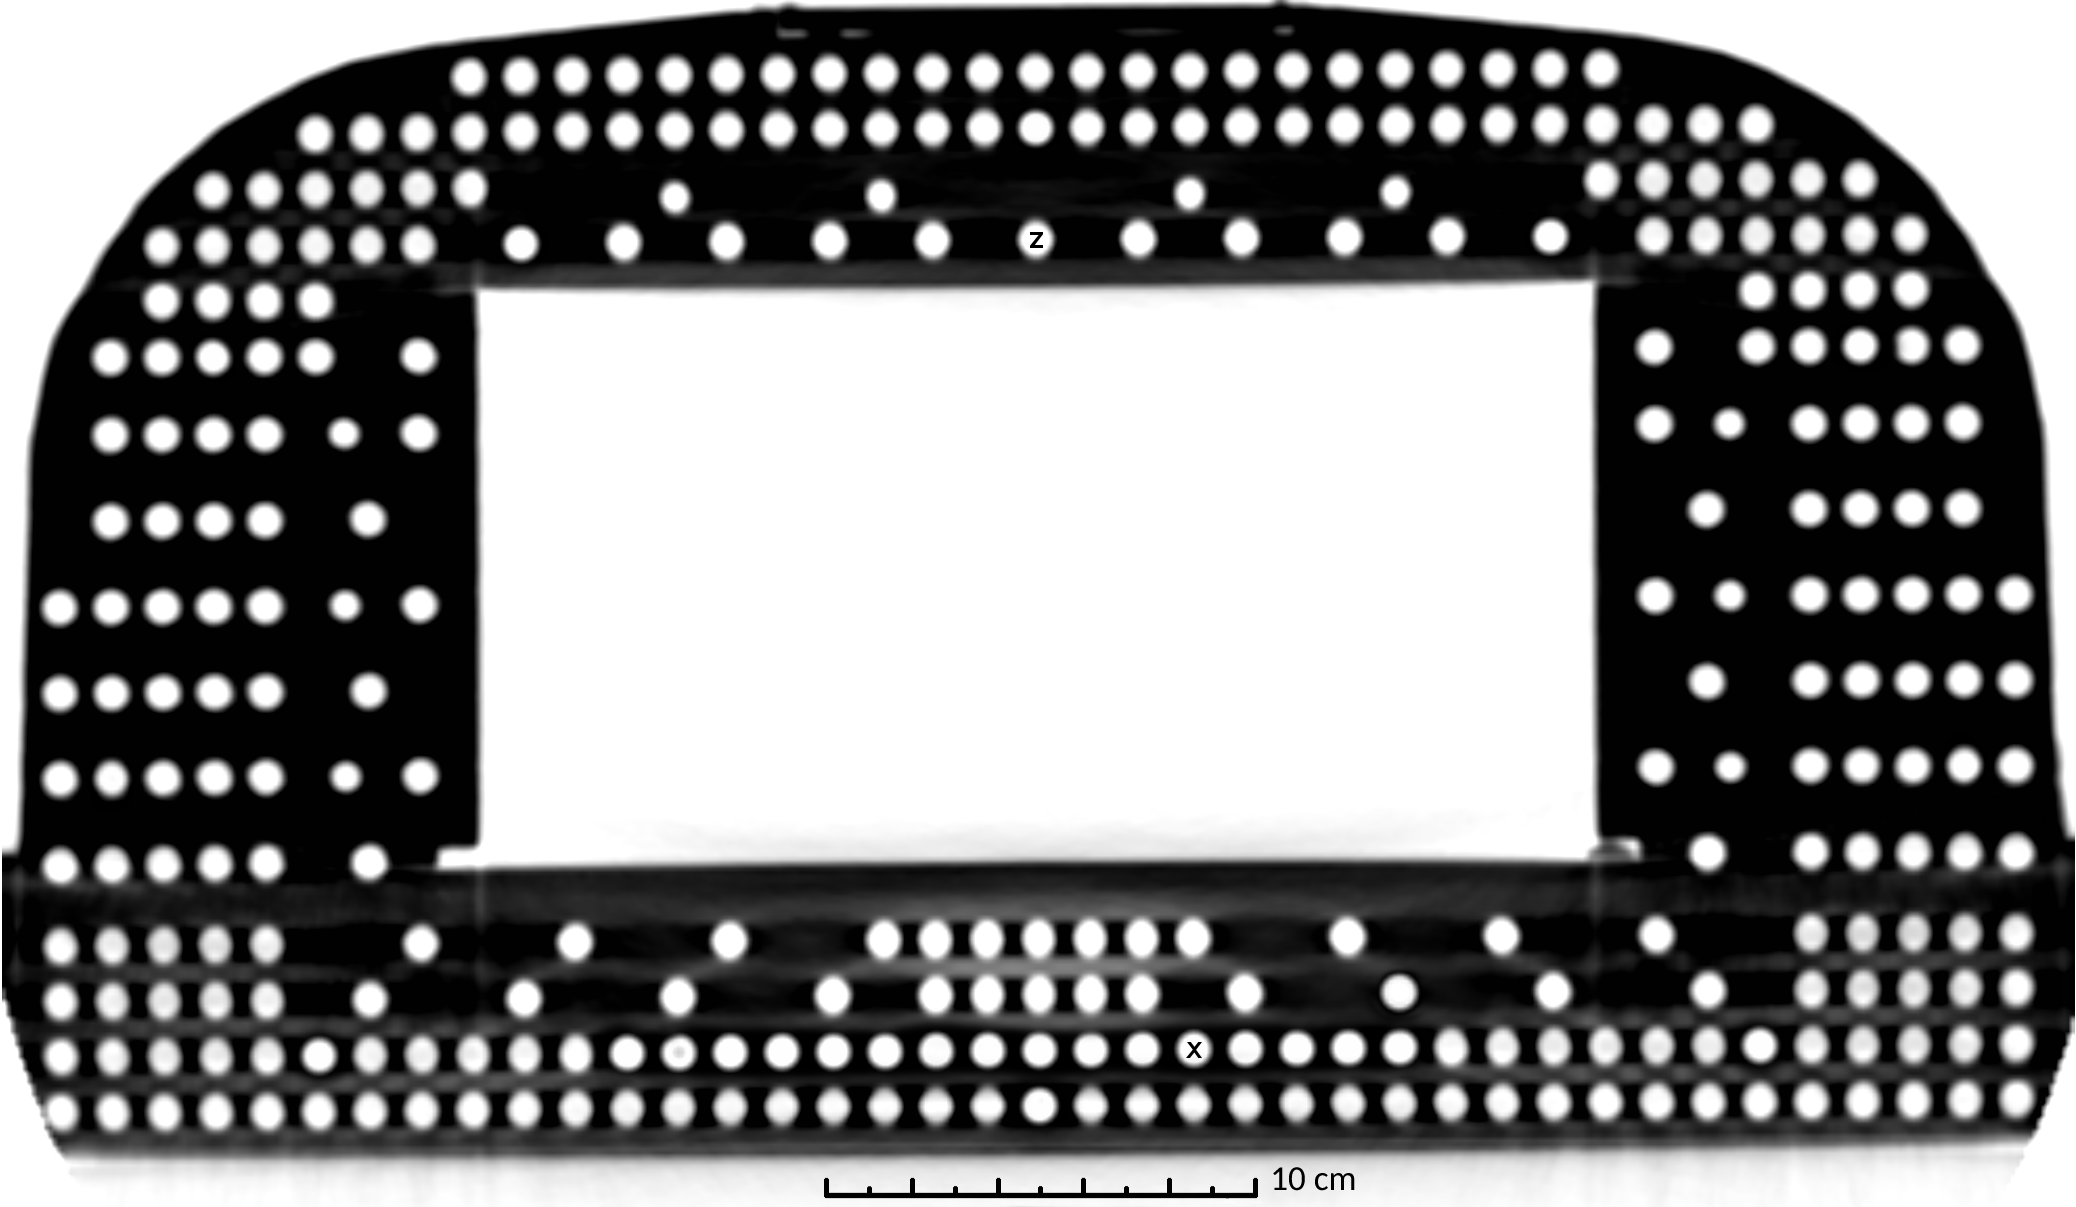
\includegraphics[width=\textwidth]{slicer3D/full_phantom/axial_CT_pane.png}
\caption{plastic pane, no rods inserted}
\label{fig:axial_CT_pane}
\end{figure}

\begin{figure}[!tbp]
\centering
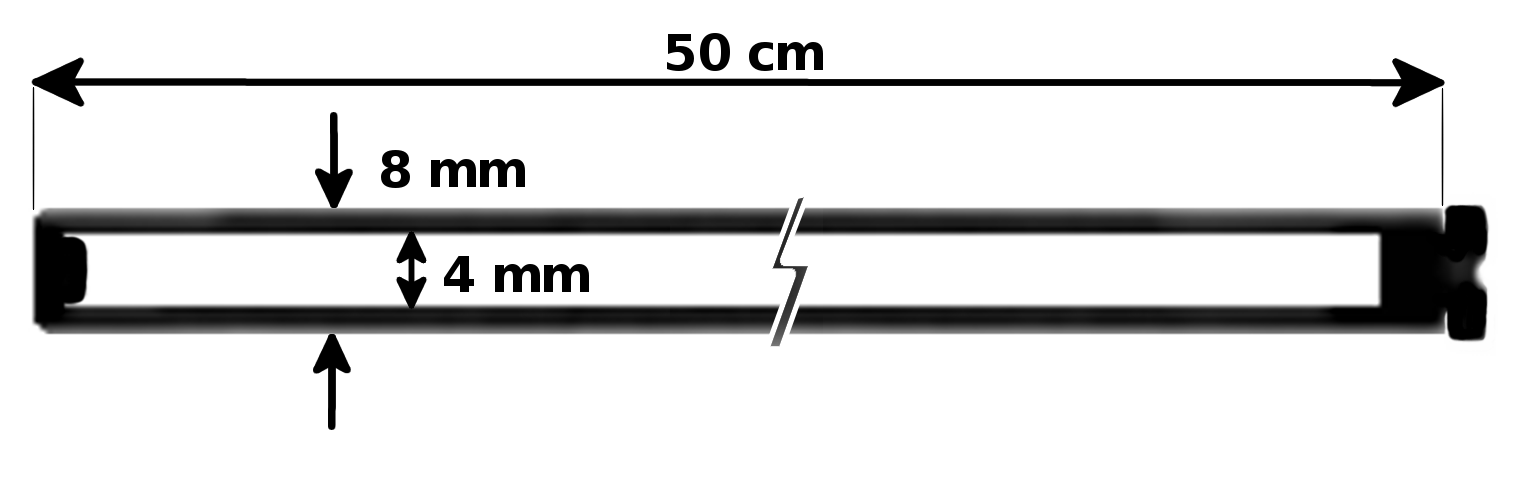
\includegraphics[width=0.8\textwidth]{slicer3D/full_phantom/rod_schematic.png}
\caption{empty plastic rod, schematic (not true proportions); }
\label{fig:rod_schematic}
\end{figure}

\vspace{4cm}
\textit{photo of Phantom}
\vspace{2cm}
\vspace{4cm}
\textit{photo of single rod}
\vspace{2cm}

\subsection{Rod fillings}

For this study 17 different liquids were produced to be tested as possible fillings.
They are listed in Table \ref{tab:solutions}.


\begin{table}[!hbt]
\centering
\begin{tabular}{@{}l|rrrrrr@{}}
No.   & $NaCl$   & $CuSO_4\cdot5H_2O$          & Soap & Ascorbic Acid & Agar & Primovist [volume-\%]\\
\toprule
\#1  &             &                   &      &               &           &		\\
\#2  & 3.6         & 1.96              &      &               &           &		\\
\#3  & 3.6         & 3.92              &      &               &           &		\\
\#4  & 3.6         & 19.6              &      &               &           &		\\
\#5  & 3.6         & 1.96              & 1    &               &           &		\\
\#6  & 3.6         & 1.96              & 5    &               &           &		\\
\#7  & 3.6         & 1.96              & 20   &               &           &		\\
\#8  & 3.6         & 1.96              &      & 0.36          &           &		\\
\#9  & 3.6         & 1.96              &      & 3.6           &           &		\\
\#10 & 3.6         & 1.96              &      & 36            &           &		\\
\#11 & 3.6         &                   &      &               &           & 0.1\%	\\
\#12 & 3.6         &                   &      &               &           & 1\%		\\
\#13 & 3.6         &                   &      &               &           & 10\%	\\
\#14 & 3.6         & 1.96              &      &               &  0.5      &		\\
\#15 & 3.6         & 1.96              &      &               &   20      &		\\
\midrule
\#16 & \multicolumn{2}{r}{Motor Oil:}   & \multicolumn{4}{l}{\textit{Castrol Power1}}      \\
\#17 & \multicolumn{2}{r}{Silicon Oil:} & \multicolumn{4}{l}{\textit{Charge: 15HLVY023}}   \\ \bottomrule
\end{tabular}
\caption{composition of tested solutions\\(components in $g/L$; exception: Primovist in volume-\%)}
\label{tab:solutions}
\end{table}

\newpage
\begin{enumerate}[label=\textbf{\#\arabic*}]
 \item \textit{distilled water} (as reference)
 \item $NaCl$ + $CuSO_4\cdot5H_2O$ (as suggested by AAPM MR Subcommittee \cite{Jackson2009})
 \item increased concentration of $CuSO_4\cdot5H_2O$
 \item further increased concentration of $CuSO_4\cdot5H_2O$
 \item generic washing-up \textit{soap} added to \textbf{\#2} (suggestion by Data Spectrum Corporation \cite{bubbles})
 \item increased \textit{soap} concentration
 \item further increased \textit{soap} concentration
 \item \textit{ascorbic acid} added to \textbf{\#2} (suggested by \cite{Abtahi2008, Bodannes1979} Concentration of $0.36 \; g/L$ corresponds to approx. $0.00204 \; mol/L$)
 \item increased \textit{ascorbic acid} concentration
 \item further increased \textit{ascorbic acid} concentration
 \item \textit{Primovist} (a common contrast agent used for MRI scans \cite{VanBeers2012, Rohrer, primovist})
 \item increased amount of \textit{Primovist}
 \item further increased amount of \textit{Primovist}
 \item \textit{agar} (or agarose is commonly used as basic reference material for MRI phantoms \cite{BuccioliniCiraolo1989, Mathur-DeVre1985})
 \item increased \textit{agar} concentration
 \item synthetic motor oil
 \item silicon oil
\end{enumerate}

% why those solutions??

Being closed at one end and having a capillary shape (small diameter) makes it impossible for the rods to be filled by pouring in the liquid.
Instead of adding the fluid at the top, it has to be injected starting at the bottom.
This way the contained air would be pushed out by the injected liquid through the opening at the top.
A thin plastic tube was inserted and used for injection, leaving enough room for the gas to escape.
Between injections of different liquids, the tube was flushed with \textbf{\#1} (distilled water) or \textbf{\#2} (main component of most solutions).

In order to minimise the amount of gas dissolved, the liquids were brought to boil shortly before injecting. Gas solubility generally decreases with rising temperature \cite{Henry1803, Sander2015}.
After injecting the solution in the rods, they were left to cool down.
Before closing, the rods were topped up completely (no trapped air bubbles).
The oil based liquids, \textbf{\#16} and \textbf{\#17}, were not brought to boil.
Number \textbf{\#14} could be injected without problems, the solution remained fluid even after reaching room temperature.
Number \textbf{\#15} on the other hand changed to a gel like consistence and clogged the tube right after the rod was filled. The tube could not be used again.



\section{Sequences}
\todo{elaborate!}
Following the suggestions given in the Report of AAPM MR Subcommittee TG1 ``MR Acceptance Testing and
Quality Control'' \cite{Jackson2009}, T1 weighted sequences were chosen to evaluate the possible solutions. (Table \ref{tab:settings})

\begin{table}[h]
\centering
\begin{tabular}{@{}lllll@{}}
System & ---  & --- &  --- & --- \\
\toprule
MRI    & -   & -   & -   & -    \\
CT     & -   & -   & -   &
\end{tabular}
\caption{used sequences}
\label{tab:settings}
\end{table}

\section{Developed software tool}

In order to asses the distortion of the MRI scanner, a tool was programmed.
It is written in Python 2.7 and uses the \textit{SimpleITK} package to read and process \textit{DICOM} (``\textit{Digital Imaging and Communications in Medicine}'') files. \cite{Python, DICOM}
\textit{SimpleITK} is a object-oriented ``C++ library with wrappers for Python, Java, CSharp, R, Tcl and Ruby''. \cite{SimpleITK, SimpleITK_started} It's versatility is one of the reasons why this approach was favoured.
It is a simplified layer built on top of the National Library of Medicine Insight Segmentation and Registration Toolkit (ITK). SimpleITK is also used by Applications like \textit{3D Slicer} , a ``free and open source software package for
visualisation and medical image computing''. \cite{3DSlicer, Kikinis2012} For this work 3D Slicer was used to crop images, quickly read values and visualise the results.
Documentation and code examples of SimpleITK can be found at \cite{InsightSoftwareConsortium, Kyriakou-SimpleITK}
An alternative way to handle DICOM data in Python would be Pydicom. \cite{Pydicom, Kyriakou-Pydicom-VTK} 

An extensive list of packages used to process data:
\begin{itemize}
 \item SimpleITK
 \item numpy
 \item scipy
 \item matplotlib.pyplot \cite{Hunter2007}
 \item skimage.draw
 \item datetime
 \item os
\end{itemize}

\subsection{Processing MRI and CT scans}

% what application used to align CT and MRI
Prior to analysing their data, the scans had to be prepared.
To start with, they were aligned in a way that yields maximum overlap especially in the centre of the image.
However, the MRI image had a lower resolution than the CT scan.
Therefore, the MRI voxel's size were changed to match the CT voxels. Both images were resampled to CT resolution.
Those steps were performed using \textit{MIRADA} (?????).

As described later, resolution might influence the efficiency of the distortion assessment.
The application \textit{3D Slicer} (Version: Slicer-4.5.0-1-linux-amd64) was used to again resample both images to a finer resolution.

Pixel spacing in x and y direction are equal. The z-axis, which lies approximately parallel to the phantom's rods, has a different pixel spacing.
Overall image resolution could have a significant effect on the results. Therefore all calculations were made using original and interpolated (increased resolution) scans.
See table \ref{tab:spacing} for more details. Figure \ref{fig:resample} depicts 3 CT/MRI scans of a single rod (axial) with different resolutions.
``x1'' stands for the original CT scan resolution (MRI resampled to match).
``x4'' is a resolution resulting in 1 pixel being split in 4 smaller pixels, ``x9'' in 9, and so on and so forth.
For better visibility, images shown as figures in this work are printed with inverted colours.
Dark pixels have a high density/intensity value, white pixels are equivalent to air (low density/intensity).

\begin{table}[!htb]
\centering
\begin{tabular}{l|l|l|l}
resample factor  & z (not affected) &  y (same as x) & x \\
\toprule
x1     & 0.60 & 0.99	& 0.98	\\
x4     & 0.60 & 0.49	& 0.49	\\
x9     & 0.60 & 0.33	& 0.33	\\
% x16    & 0.60 & 0.244	& 0.24	\\
x25    & 0.60 & 0.2 	& 0.2	\\
x100   & 0.60 & 0.2 	& 0.1
\end{tabular}
\caption{pixel Spacing (rounded values) [$mm$]}
\label{tab:spacing}
\end{table}


\begin{figure}[!thb]
  \begin{subfigure}[b]{0.32\textwidth}
    
\includegraphics[scale=.11]{slicer3D/profiles/CT_x1.png}
    \caption{CT x1}
    \label{fig:CT_x1}
  \end{subfigure}
  \hfill
  \begin{subfigure}[b]{0.32\textwidth}
    
\includegraphics[scale=.11]{slicer3D/profiles/CT_x9.png}
    \caption{CT x9}
    \label{fig:CT_x9}
  \end{subfigure}
    \hfill
  \begin{subfigure}[b]{0.32\textwidth}
    
\includegraphics[scale=.11]{slicer3D/profiles/CT_x100.png}
    \caption{CT x100}
    \label{fig:CT_x100}
  \end{subfigure}
  \begin{subfigure}[b]{0.32\textwidth}
    
\includegraphics[scale=.11]{slicer3D/profiles/MR_x1.png}
    \caption{MRI x1}
    \label{fig:MRI_x1}
  \end{subfigure}
  \hfill
  \begin{subfigure}[b]{0.32\textwidth}
    
\includegraphics[scale=.11]{slicer3D/profiles/MR_x9.png}
    \caption{MRI x9}
    \label{fig:MRI_x9}
  \end{subfigure}
    \hfill
  \begin{subfigure}[b]{0.32\textwidth}
    
\includegraphics[scale=.11]{slicer3D/profiles/MR_x100.png}
    \caption{MRI x100}
    \label{fig:MRI_x100}
  \end{subfigure}
  \caption{CT/MRI: axial image of single rod, filling \#5  (inverted colours)}
  \label{fig:resample}
\end{figure}
\clearpage



\subsection{Capabilities}

The developed software tool is not able to automatically detect individual rods shown in a CT or MRI scan.
Instead the acquired 3D images have to be cropped to depict only a single rod.

The python script can:
\begin{itemize}
 \item denoise the image data
 \item find the brightness values of the rod, enabling it to
 \item separate pixels representing the rod from surrounding air (masking)
 \item calculate the centroid coordinates along the rod, used to
 \item calculate the local distortion
  \subitem location shift
  \subitem dice coefficient (roundness/deformation)
 \item plot individual rod slices
  \subitem overlaying one or two centroid coordinates
  \subitem and save it as ``.png'' file
 \item change the pixel values to reflect the distortion occurring along a rod (visualisation)
 \item write the calculated numbers to a ``.txt'' file
\end{itemize}

\subsection{Measuring distortion}

Two phenomena were chosen to reflect the amount of distortion occurring in MRI scans:

\begin{enumerate}[label=\textbf{\arabic*)}]
 \item location shift (``warp'')
 \item deformation (deviation from circular profile ``DC'')
\end{enumerate}

Since the rods have a cylindrical shape, distortion can only be assessed in radial direction. To make calculations easier, the z-coordinate was put parallel to the rods, x and y radial.
Each slice (z = const.) should ideally depict the bright circular profile of the liquid (+ plastic rod in CT) surrounded by black (air).
To calculate the location shift between rods shown in CT and MRI, the coordinates of the centre of mass (COM) were subtracted.
The location difference in each slice is saved as an array. Additionally, the absolute value of the coordinate shift (absCS) could be calculated.

% image of COM shift

The dice-coefficient ``DC'' (also known as Sorensen-Index) was chosen as indicator for the deviation from a circular profile. Again this value was calculated for every slice using either the CT or MRI scans.

To get a idea of the occurring distortion one should look at both the absolute value of coordinate shift and the dice-coefficient (DC).
The DC ranges from 0 to 1. A value of 1 indicates a perfect circular shape. A low DC on the other hand could be caused by many things such as:
little overlap (e.g. a ring or crescent shape); a very dark image hindering delineation of rod from background; a small circle with a radius close to a only a few pixels.


% A proposed third indicator combining warp magnitude and the DC:
% $warpDC = warpMagnitude * (1-DC)$

\subsection{Calculation: dice-coefficient (DC)}

The dice coefficient or Sorensen index \cite{MedPy_dc-doc} is defined as:

\begin{align}
DC = \frac{2 |A \, \cap \, B|}{|A| + |B|}
\end{align}

The implementation into python is based on the open source python package ``Medpy''. \cite{MedPy} A part of it's module called ``metric'' was adapted. \cite{MedPy_dc-code}
All pixels above a certain threshold will be counted as input A. The reference B is a circle whose midpoint is placed at the centre of mass (COM).

The calculation of the DC is done by comparing an binary image to a circle. The position of the circle's centre and its radius is highly influencing the outcome.
Both the circle's centre and its radius were varied during the distortion assessment.


\subsection{Calculation: center of mass (COM)}

The calculation of the COM is done with help of the ``scipy'' python package.
It's module ``ndimage'' contains the function ``$center\_of\_mass()$'', which returns the COM's coordinates of a given input array.
The values assigned to voxels in CT images lie in the range from -1024 HU (air) to around 200 HU (plastic rod).
Before a meaningful result can be obtained, the values need to be shifted to be $>$ 0.
Additionally, only pixels representing the rod or the liquid should be used for the calculation.
Otherwise the almost black voxels surrounding the rod would influence the result.
This error could be observed especially if the rod is not placed in the exact middle of the scan.
As described earlier, the plastic rod is only visible in CT images. On the MRI scans solely the liquid containded in the rods is shown. Therefore rods appear to be smaller on the MRI data.
To find the relevant pixels two algorithms were developed:

\begin{description}
 \item[1] calculating the number of pixels based on rod size
 \item[2] finding a COM resulting in good DC
\end{description}

add 1:
The inner ($4mm$) and outer ($8mm$) diameter of the rods are known. So is the \textit{pixel spacing} which represents the equivalent size of a voxel in $mm$.
Calculating the number of pixels which make up the more or less circular profile of the rod in each slice is calculated as follows:

\begin{align}
 pixelNumber = (radius^2 \cdot \pi) \, / \, (spacing^2)
\end{align}

For CT images $radius = 4mm$, in MRI scans $radius = 2mm$. $spacing$ is the pixel spacing in x and y direction.
Next the pixels are sorted by brightness. The top $pixelNumber$ pixels are then used to calculate the COM.

add 2:
This algorithm is an iteration method. It starts by assuming $\approx 50\%$ of all pixels in the image are part of the rod.
This first guess of $50\%$ is shifted by multiplying it with $(1 \pm 0.2) \rightarrow 1.2$ and $0.8$.
So in the first step two possible COMs are obtained using the brightest $50*1.2 = 60\%$ and $50*0.8 = 40\%$ of all pixels.
It takes note of the values assigned to the darkest and brightest pixels used during both calculations.
Those values are then set as threshold for the DC coefficient.
Effectively it finds COM and DC for $52\%$ and $60\%$. If the DC for using 52\% is bigger, it chooses $(100\% + 50\%) / 2 = 75\%$ as next guess.
If on the other hand the DC for $40\%$ is bigger, it chooses $(0\% + 50\%) / 2 = 25\%$ as next guess.
In the second iteration it now again shifts the percentage by multiplying it with $1.2$ and $0.8$. Again COM and DC are calculated and the next guess is chosen by comparing the DCs.
This is continued until the DC value decreases compared to DC found in prior steps. The maximum DC is used as indicator for the best COM.

% image of COM shift
\todo{flowchart for algorithms (send handwritten draft to Piotr)}


\chapter{Results}
% o Present all results here
% o No discussion, no interpretation, no evaluation etc.
% o Figures / Tables
%  Use wisely
%  Consult your supervisor about what to present
%  put very large and detailed tables rather in the appendix
%  put source code in appendix
% o Do not write down all data from table in text, but put them in relation to each other
% o Help reader to understand tables & graphs and highlight important and/or interesting data
% o Present an assessment of uncertainties

On the second day of working with the filled rods the one containing liquid \textbf{\#6} broke (leakage).
It happened when delicately knocking it against on the table while standing upright.
This was intended to mobilise bubbles that sticked to the wall and make them travel vertically to on end of the rod. (see tabular \ref{tab:bubbles})
The plastic stopper on the lower end came loose.
The rod containing filling \textbf{\#6} was not replaced.
Consequently, all CT and MRI images show only 16 rods.

\section{Obtained MRI and CT scans}
Figure \ref{fig:coronal} shows a coronal view of the 16 rods filled with the tested liquids.
(in figure \ref{fig:axial_MR} a plastic bottle filled with water has been placed there instead (see figure \ref{fig:axial_CT_pane}).)
 
\begin{figure}[!tbp]
  \begin{subfigure}[b]{\textwidth}
    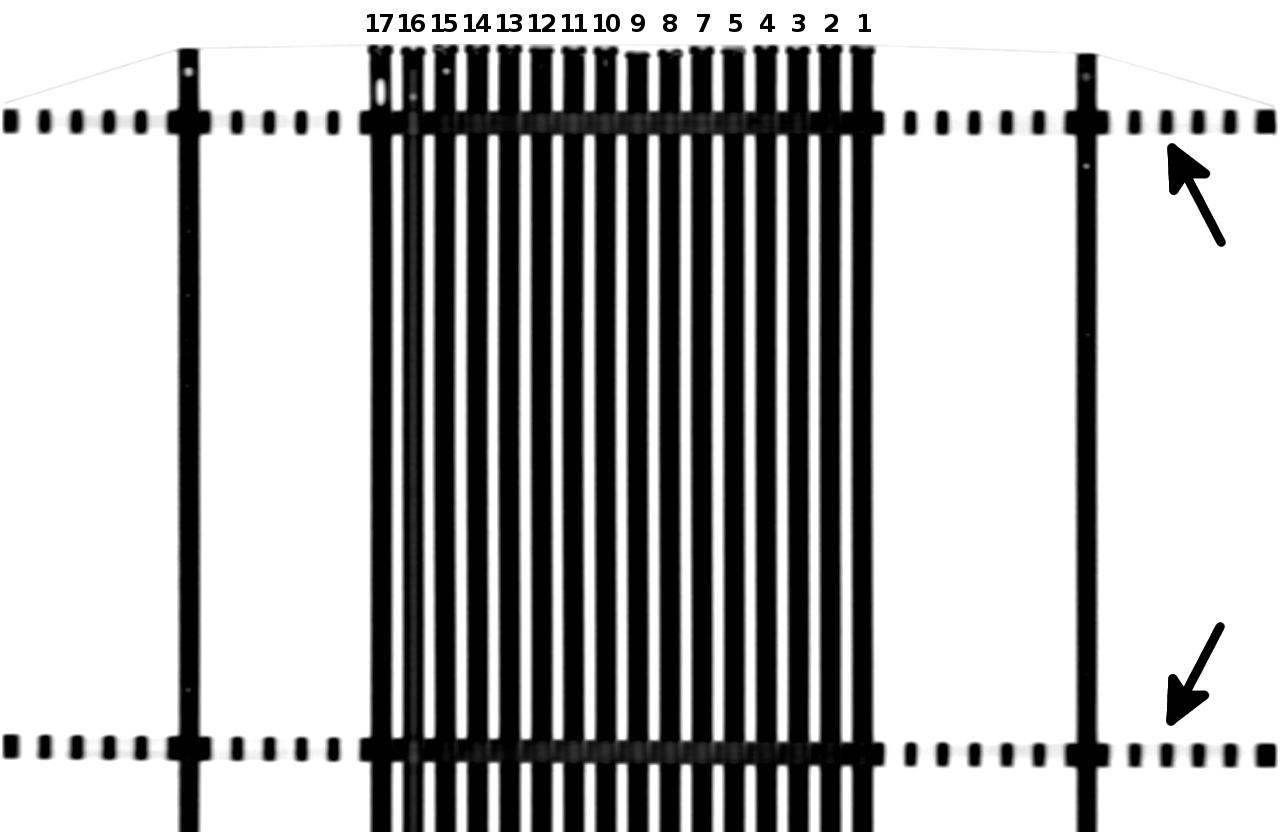
\includegraphics[width=\textwidth]{slicer3D/full_phantom/coronal_CT_cropped-arrow.png}
    \caption{CT: periodic black lines in upper and lower part of image (arrows) show plastic panes from above); rods have been fixed with adhesive tape (faint line across upper end of rods); differences in signal intensity (brightness) hardly noticeable, but air bubbles visible at upper end}
    \label{fig:coronal_CT}
  \end{subfigure}
  \begin{subfigure}[b]{1\textwidth}
    
\includegraphics[width=1\textwidth]{slicer3D/full_phantom/coronal_MR_cropped.png}
    \caption{MR: rods appear to be thinner, because only the liquid filling is visible; plastic (rods and panes) are not visible}
    \label{fig:coronal_MR}
  \end{subfigure}
  \caption{Coronal CT/MRI (inverted colours; same scale; cropped images): images of 16 rods (tested liquids, numbering starting from the right, \#6 excluded) + 2 reference rods (filled with water) on the sides; liquids result in different signal intensity (brightness)}
  \label{fig:coronal}
\end{figure}

\begin{figure}[!tbp]
  \begin{subfigure}[b]{\textwidth}
    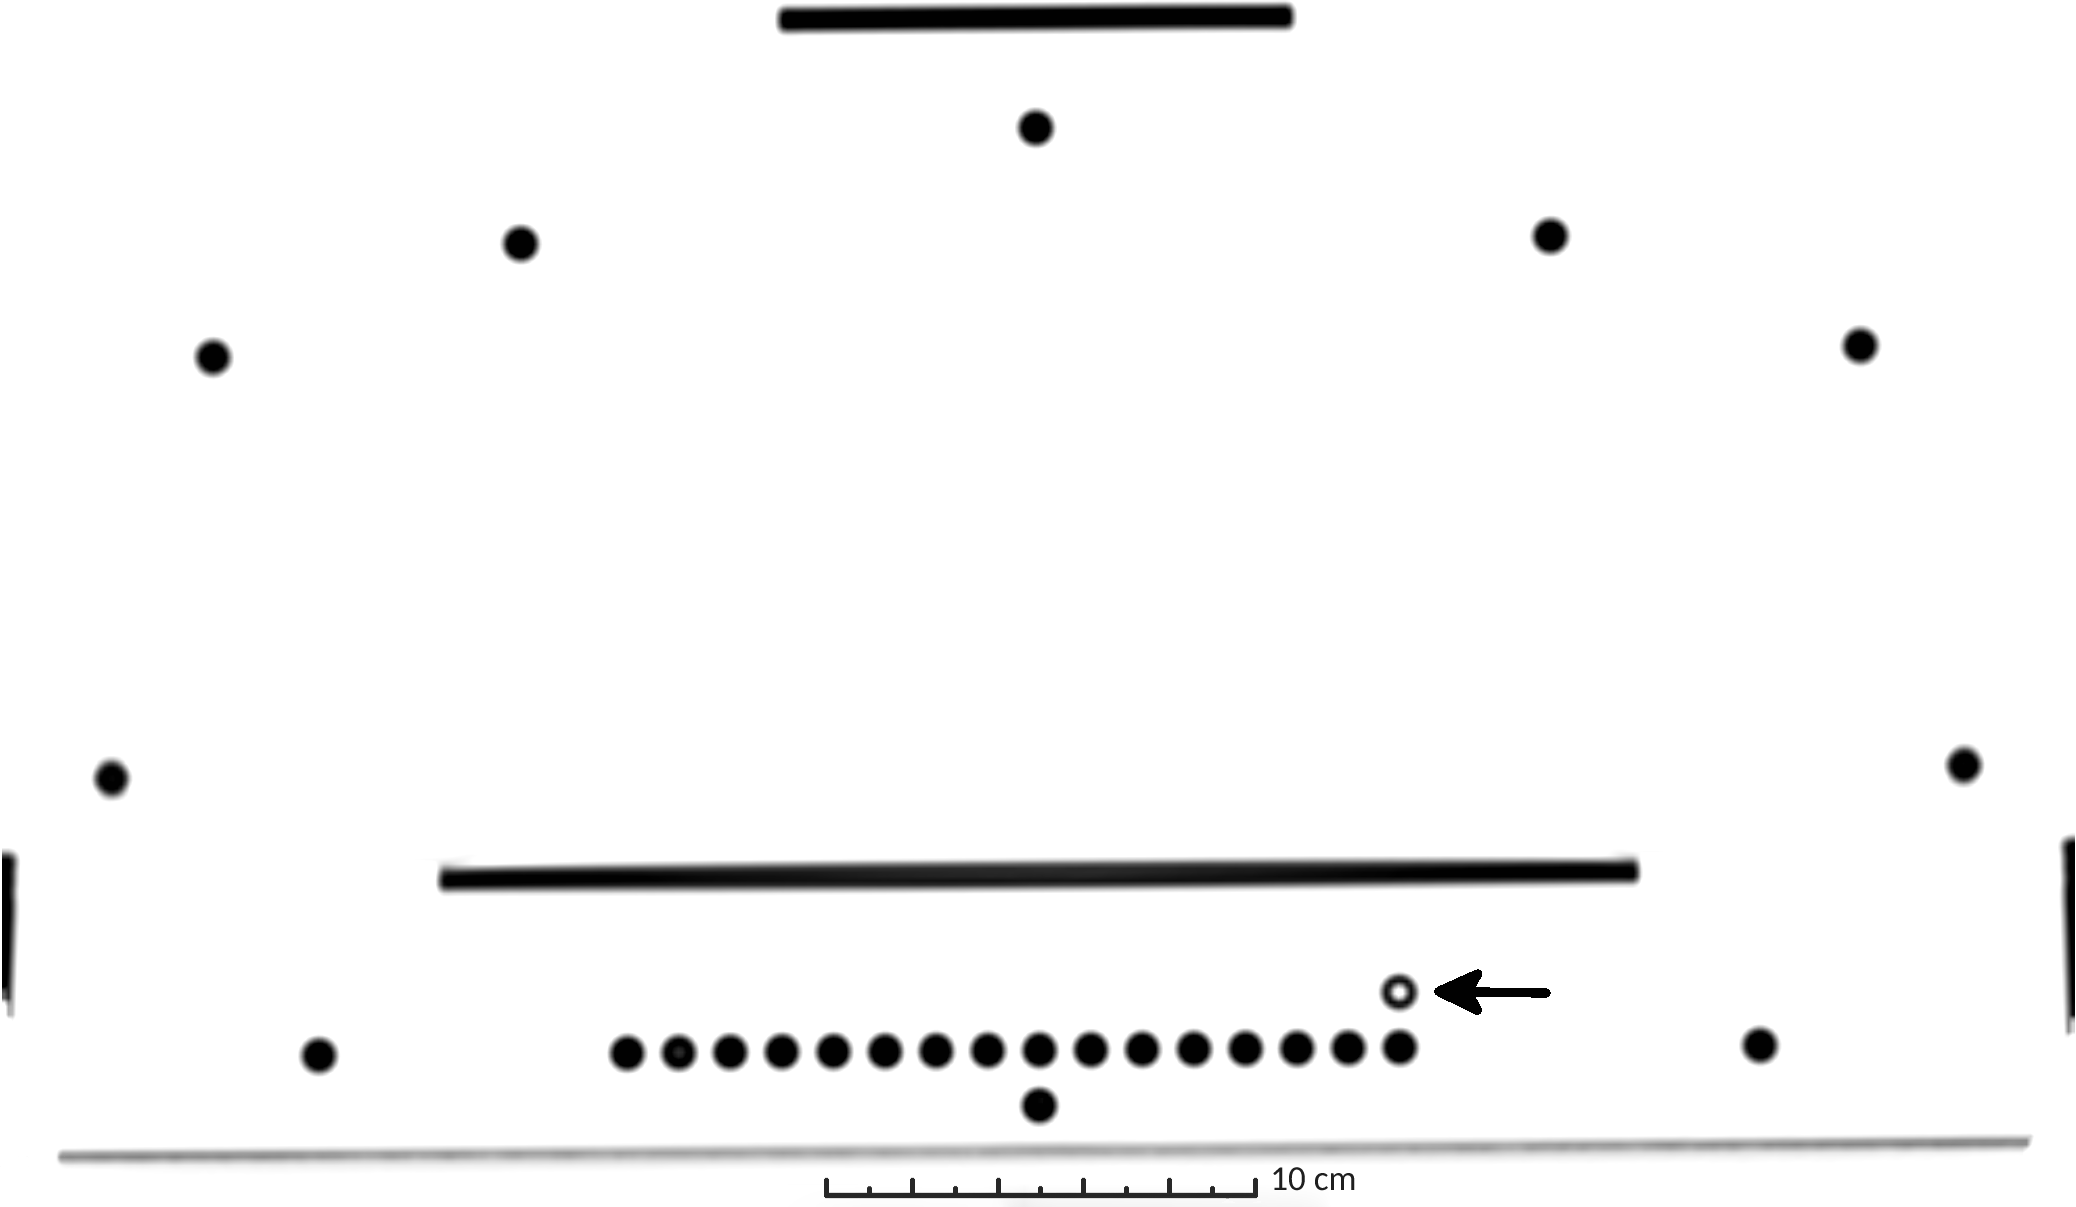
\includegraphics[width=\textwidth]{slicer3D/full_phantom/axial_CT_rods-arrow.png}
    \caption{CT: black bars just above tested rods, at the very top and to the sides show plastic parts of the phantom holding it together; faint grey line below tested rods shows table on which phantom was positioned during imaging}
    \label{fig:axial_CT_rods}
  \end{subfigure}
  \begin{subfigure}[b]{\textwidth}
    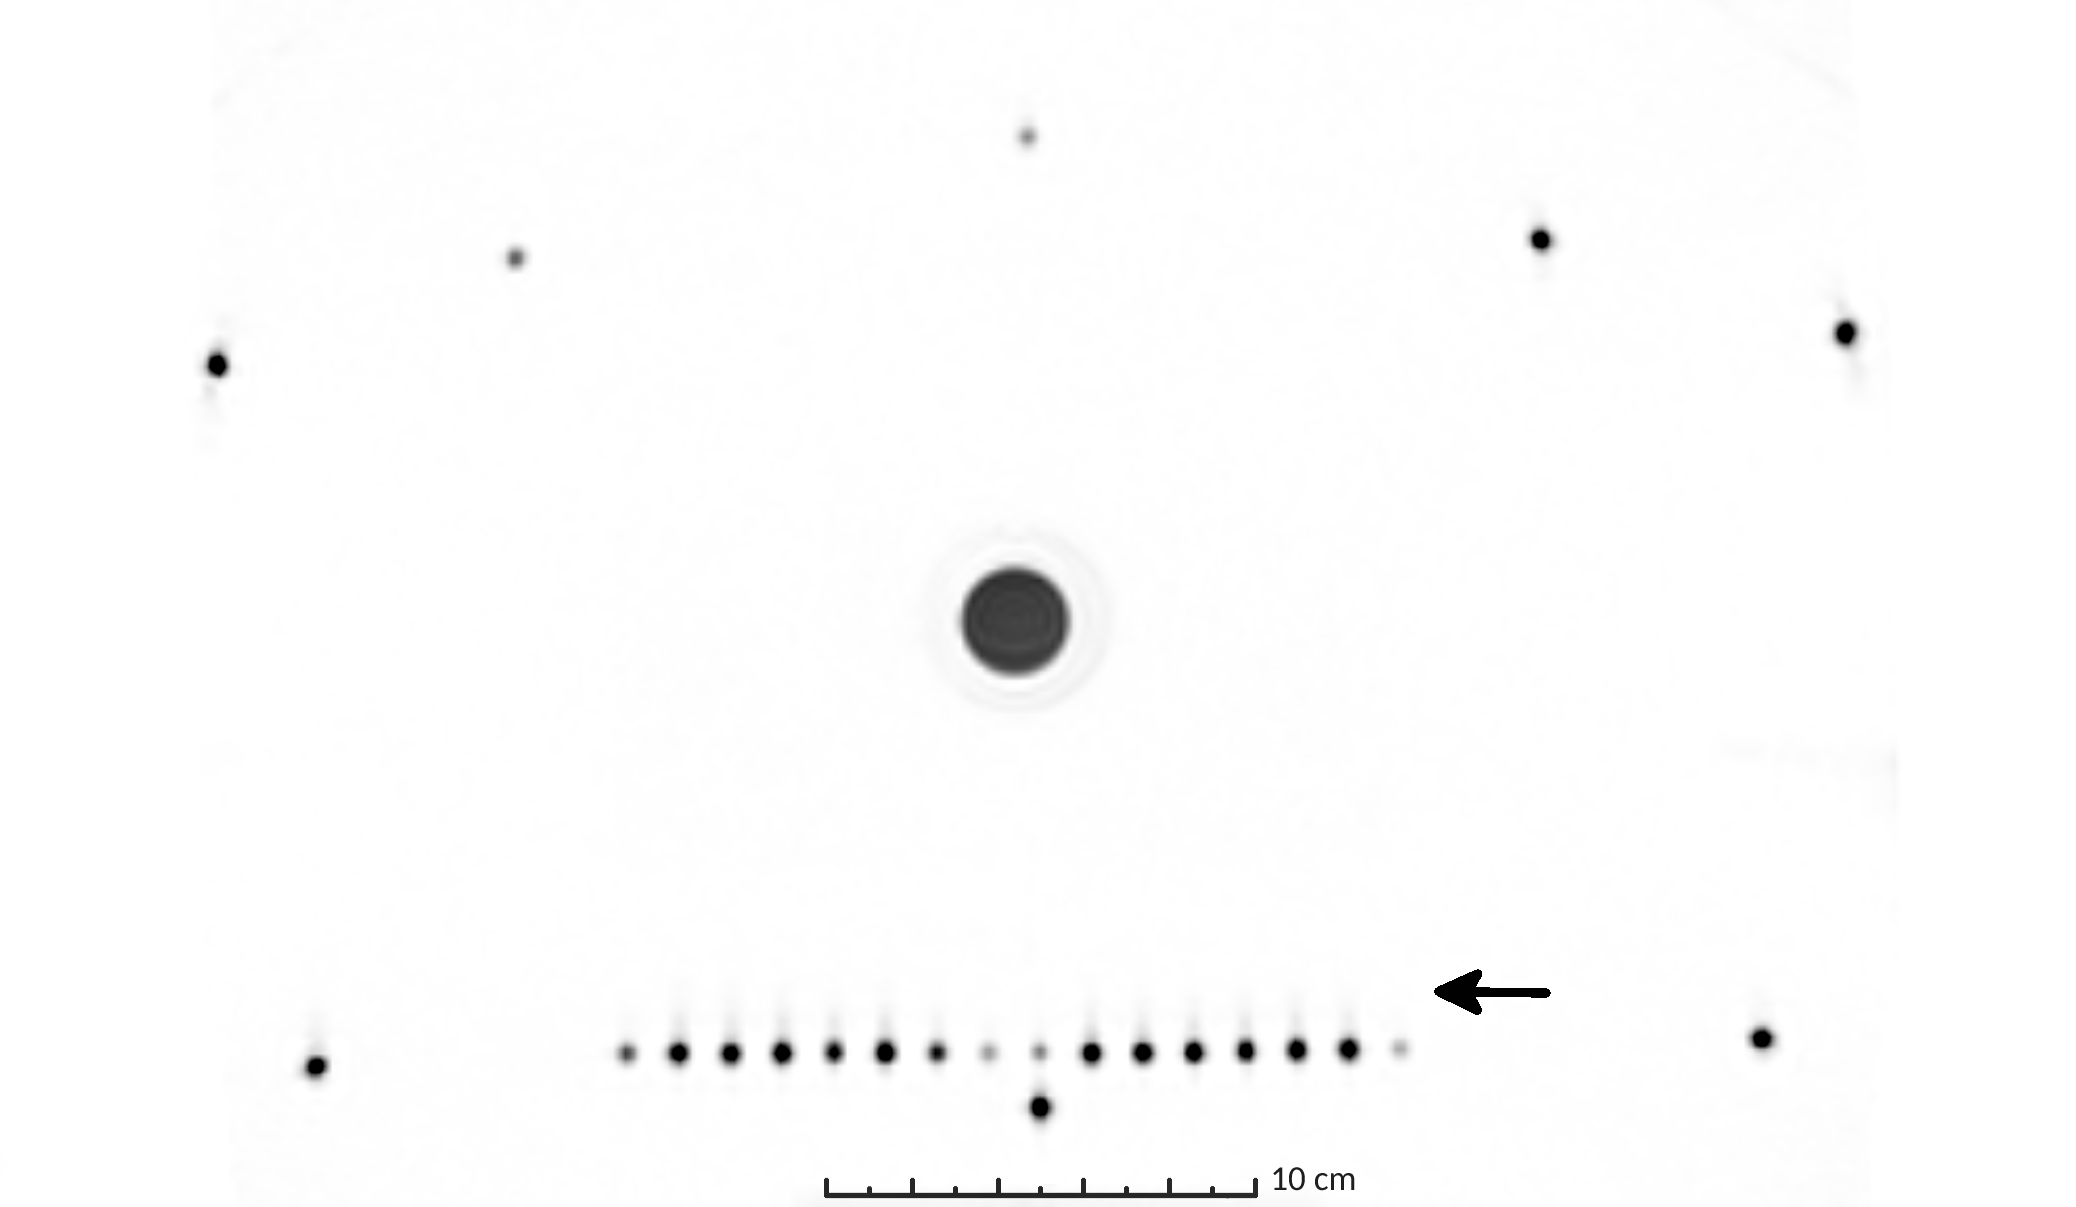
\includegraphics[width=\textwidth]{slicer3D/full_phantom/axial_MR-arrow.png}
    \caption{MRI: black circle in middle shows water bottle which was placed in the middle of the phantom (necessary for MRI scanner to start imaging)}
    \label{fig:axial_MR}
  \end{subfigure}
  \caption{axial CT/MRI (inverted colours, same scale): images of 16 rods (tested liquids, numbering starting from the right, \#6 excluded); surrounded by reference rods (filled with water) and one empty rod (marked with arrow) which is not visible on MRI scans}
  \label{fig:axial}
\end{figure}


\section{Tested solutions}

\subsection{Visibility on CT/MRI scans}

CT images show little differences between the tested liquids. The plastic rods themselves result in brighter pixels than any of the tested solutions.

On MRI scans most liquids had a mean and a max brightness value above $1000$ (see table \ref{tab:visibility}).\\
Only \textbf{\#1}, \textbf{\#9}, \textbf{\#10}, \& \textbf{\#17} resulted in significantly less signal (below < $1000$).


\begin{table}[!htb]
\centering
\begin{tabular}{@{}lllllll@{}}
\toprule
No. & Min  & Max  & Mean   & Median & RMS    & $\sigma$   \\ \midrule
1   & 182  & 371  & 288    & 269    & 296,3  & 69,8   \\
2   & 1044 & 1921 & 1443,8 & 1405   & 1477,3 & 312,9  \\
3   & 941  & 2075 & 1451,2 & 1394,5 & 1508,9 & 413,2  \\
4   & 1176 & 1709 & 1440   & 1437,5 & 1458,6 & 232,5  \\
5   & 1125 & 2111 & 1583,8 & 1549,5 & 1623   & 355    \\
7   & 971  & 2241 & 1466,8 & 1316   & 1540,6 & 471,2  \\
8   & 1459 & 1947 & 1704   & 1705   & 1713,5 & 180,5  \\
9   & 385  & 584  & 486,8  & 489    & 495,6  & 93     \\
10  & 247  & 502  & 343,6  & 266    & 361,1  & 111    \\
11  & 830  & 1268 & 1036,2 & 1023,5 & 1049   & 163,2  \\
12  & 1158 & 2211 & 1648,8 & 1613   & 1695,2 & 394,2  \\
13  & 836  & 1657 & 1146,8 & 1047   & 1190,9 & 321,2  \\
14  & 800  & 2062 & 1383   & 1335   & 1461,7 & 473,1  \\
15  & 1156 & 1829 & 1476,2 & 1460   & 1501,2 & 272,7  \\
16  & 1102 & 1967 & 1509   & 1483,5 & 1543,8 & 325,8  \\
17  & 356  & 938  & 629,6  & 602    & 668,1  & 223,6  \\ \bottomrule
\end{tabular}
\caption{liquid visibility on MRI scan}
\label{tab:visibility}
\end{table}

\clearpage

\subsection{Mechanical properties of solutions}
\label{sec:sol-mech}

The liquids were filled in a rod each and observed for several months.
Number \textbf{\#14} could be injected without problems, the solution remained fluid even after reaching room temperature.
Number \textbf{\#15} on the other hand changed to a gel like consistence and clogged the injection tube at the quickly after the rod was filled.
The tube could not be used again.

Each rod was free of bubbles directly after sealing.
All rods containing water based solutions contained some air after 2 months and the amount of liquid continued to decrease further (see table \ref{tab:bubbles}).
In some of the tested rods the produced air bubbles would stick to the wall. Only after gently hitting the rod they would start moving.
Knowing the inner diameter $d$ of the rods and measuring the length $l$ of trapped air bubbles, we can approximate the volume of contained gas:

\begin{align}
 V = \frac{d^2}{4}\cdot \pi \cdot l
\end{align}

\begin{table}[]
\centering
\begin{tabular}{l|lc|lc|lc}
    & \multicolumn{2}{c}{\textit{after 1 day}} 	& \multicolumn{2}{c}{\textit{after 2 days}}	& \multicolumn{2}{c}{\textit{after 1 week}}	\\ 
No. & bubbles	& hit req.	& bubbles 	& hit req.	& bubbles 	& hit req.	\\
\toprule
\#1   & yes	& no		& no		&		& no		&		\\
\#2   & yes	& yes		& no		&		& no		&		\\
\#3   & yes	& yes		& no		&		& no		&		\\
\#4   & yes	& yes		& no		&		& no		&		\\
\#5   & yes	& no		& yes		& no		& no		&		\\
\#6   & yes	& no		& \multicolumn{4}{l}{-----------------\textit{ rod was leaking }------------------}	\\
\#7   & yes	& no		& yes		& no		& yes		& no		\\
\#8   & no	&		& no		&		& no		&		\\
\#9   & no	&		& no		&		& no		&		\\
\#10  & no$^1$	&		& yes		& yes		& yes		& yes		\\
\#11  & no	&		& yes,		& \textit{sticked to wall} &	 yes	& yes\\
\#12  & yes	& yes		& yes,		& \textit{sticked to wall} &	 yes	& yes\\
\#13  & yes	& yes		& yes,		& \textit{sticked to wall} &	 yes	& yes\\
\#14  & no	&   		& yes		& no		& yes		& yes		\\
\#15  & no	&   		& no		&		& no		&		\\
\#16  & no	&   		& no		&		& no		&		\\
\#17  & no	&   		& no		&		& no		&		\\
\bottomrule
\end{tabular}
\begin{tabular}{l|lr}
\multicolumn{3}{c}{}								\\
& \multicolumn{2}{c}{\textit{after 2 months}}					\\ 
No. & length of trapped bubble $l$ [$mm$] 	& approx. volume $V$ [$mm^3$]	\\
\toprule
\#1   & 2					& 25.13				\\
\#2   & 1.8					& 22.62				\\
\#3   & 1+1 (air blockage, at lower end)	& 25.13				\\
\#4   & 4					& 50.27				\\
\#5   & 1.5 (many small bubbles)		& 18.85				\\
\#6   & \multicolumn{2}{c}{-----------------------------\textit{ rod was leaking }------------------------------}\\
\#7   & 2 (many small bubbles)			& 25.13				\\
\#8   & 2.3					& 28.90				\\
\#9   & 3					& 37.70				\\
\#10  & 2.4					& 30.16				\\
\#11  & 2					& 25.13				\\
\#12  & 2					& 25.13				\\
\#13  & 2.3					& 28.90				\\
\#14  & 1.5+0.5 (big immobile bubble, at center)	& 25.13				\\
\#15  & 3.4 (agar gel dried)			& 42.73				\\
\#16  & 0					& 0.00				\\
\#17  & 0.5					& 6.28				\\
\bottomrule
\end{tabular}
\caption{solutions, observations}
\label{tab:bubbles}
\end{table}


While adding generic washing soap (\textbf{\#5}, \textbf{\#6}, and \textbf{\#7}) did not hinder air bubbles from forming, it significantly improved their mobility.
Not only did they move quickly when the rod was tilted, large quantities of air also did not block the entire diameter of the rod.
Instead they formed large but cohesive bubbles that could be moved to one end of the rod easily and at no point sticked to the plastic wall.

The ascorbic acid present in \textbf{\#8} (concentration of $0.36 \; g/L$ corresponds to approx. $0.00204 \; mol/L$), \textbf{\#9} ($3.6 g/L$), and \textbf{\#10} ($36 g/L$) seemed to have held back the formation of air bubbles for up to one week.
After two months of observation, however, the rods also contained some air.
It should be noted that all three liquids turned brown, the colour being more saturated for higher concentrations of ascorbic acid.

The rods filled with Primovist (\textbf{\#11} to \textbf{\#13}) were filled with some air bubbles after at least two days.
Moreover, the bubbles sticked to the walls of the rod and only shaking it violently made them move to one side of the rod.

It took more than a week until the rod containing the low concentration of agar (\textbf{\#14}) contained an air bubble.
The viscous consistency made it impossible to coerce it to either end of the rod.
Liquid \textbf{\#15} on the other hand did not form bubbles at the middle of the rod, but seemed to have dried starting at the end with the plastic stopper.

% \begin{table}[p]
%   \centering
%   \rotatebox{90}{
%     \begin{minipage}{\textheight}\footnotesize
%       \centering
%       \begin{tabular}{@{}r|cccc|ccccrrr@{}}
% 	    & \multicolumn{4}{c}{\textit{after 1 day}}	& \multicolumn{4}{c}{\textit{after 2 days}}			& \multicolumn{4}{c}{\textit{after 1 week}}&		 \multicolumn{4}{c}{\textit{after 2 months}}                 \\ 
% 	    & \multicolumn{4}{c}{} 			& \multicolumn{4}{c}{}                             \\
% 	Nr. & bubbles	& angle		& hit req.	& bubbles 	& angle		& hit req.	&  \\
% 	\toprule
% 	1   & yes	& $10^o$	& no		& no		&		&		&   \\
% 	2   & yes	& $40^o$	& yes		& no		&		&		&   \\
% 	3   & yes	& $40^o$	& yes		& no		&		&		&   \\
% 	4   & yes	& $80^o$	& yes		& no		&		&		&   \\
% 	5   & yes	& $10^o$	& no		& yes		& $10^o$	& no		&   \\
% 	6   & yes	& $10^o$	& no		& \multicolumn{5}{r}{--------------\textit{ rod was leaking }------------} \\
% 	7   & yes	& $10^o$	& no		& yes		& $10^o$	& no		&   \\
% 	8   & no	&		&   		& no		&		&		&   \\
% 	9   & no	&		&   		& no		&		&		&   \\
% 	10  & no$^1$	&		&   		& yes		& $20^o$	& yes		&   \\
% 	11  & no	&		& yes		& yes		& \multicolumn{4}{r}{---\textit{ bubbles sticked to wall }---} \\
% 	12  & yes	& $60^o$	& yes		& yes		& \multicolumn{4}{r}{---\textit{ bubbles sticked to wall }---} \\
% 	13  & yes	& $80^o$	& yes		& yes		& \multicolumn{4}{r}{---\textit{ bubbles sticked to wall }---} \\
% 	14  & no	&		&   		& yes		& $40^o$	& no		&   \\
% 	15  & no	&		&   		& no		&		&		&   \\
% 	16  & no	&		&   		& no		&		&		&   \\
% 	17  & no	&		&   		& no		&		&		&   \\
% 	\bottomrule
%       \end{tabular}
%       \caption{Messwerte}
%       \label{tab:wirkungsgrad}
%     \end{minipage}
%   }
% \end{table}

\section{Distortion assessment}
All results were obtained by manually cropping the 3D image to depict only a single rod.
%As described later, resolution might influence the efficiency of the distortion assessment.#	
%Therefore all calculations were done with the original resolution and interpolated images that have a higher resolution.


\begin{table}[p]
   \centering
   \rotatebox{90}{
     \begin{minipage}{\textheight}\footnotesize
       \centering
\begin{tabular}{r|lll|ll|llll|ll}
slice & $warp_x$  & $warp_y$  & $warp$ & $DC_{CT}$  & $DC^*_{CT}$ & $DC_{MR}$  & $DC^*_{MR}$ & $DC_{MR(CT-COM)}$ & $DC^*_{MR(CT-COM)}$ & $warpDC$ & $warpDC^*$ \\
\hline
0      & -0.1119 & -1.0929 & 1.0986 & 0.9942 & 0.9942 & 0.9411 & 0.8619 & 0.6403 & 0.6427 & 0.0647 & 0.1517 \\
1      & -0.1283 & -1.0923 & 1.0999 & 0.9932 & 0.9932 & 0.9438 & 0.8669 & 0.6453 & 0.6474 & 0.0618 & 0.1464 \\
2      & -0.1356 & -1.091  & 1.0994 & 0.9922 & 0.9922 & 0.949  & 0.8744 & 0.6502 & 0.652  & 0.0561 & 0.1381 \\
3      & -0.1537 & -1.0799 & 1.0908 & 0.9942 & 0.9942 & 0.9466 & 0.8821 & 0.6564 & 0.6585 & 0.0582 & 0.1286 \\
: &         &         &        &        &        &        &        &        &        &        &        \\
\hline
: &         &         &        &        &        &        &        &        &        &        &        \\
169    & 0.01    & -0.6987 & 0.6988 & 0.9899 & 0.9899 & 0.9089 & 0.9515 & 0.7731 & 0.7784 & 0.0637 & 0.0339 \\
170    & 0.0085  & -0.6953 & 0.6954 & 0.9887 & 0.9887 & 0.9086 & 0.9512 & 0.7722 & 0.7775 & 0.0636 & 0.0339 \\
171    & 0.0094  & -0.6862 & 0.6863 & 0.9883 & 0.9883 & 0.9089 & 0.9509 & 0.7717 & 0.7771 & 0.0625 & 0.0337 \\
172    & 0.0158  & -0.6797 & 0.6799 & 0.9847 & 0.9847 & 0.9088 & 0.9509 & 0.7709 & 0.7763 & 0.062  & 0.0334 \\
173    & -1      & -1      & -1     & -1     & -1     & 0.9085 & 0.9505 & -1     & -1     & -1     & -1     \\
174    & -1      & -1      & -1     & -1     & -1     & 0.9089 & 0.9509 & -1     & -1     & -1     & -1     \\
: & :        & :        & :       & :       & :       &        &        & :       & :       & :       & :       \\
\hline
: & :        & :        & :       & :       & :       &        &        & :       & :       & :       & :       \\
192    & -1      & -1      & -1     & -1     & -1     & 0.914  & 0.9515 & -1     & -1     & -1     & -1     \\
193    & -1      & -1      & -1     & -1     & -1     & 0.9144 & 0.9518 & -1     & -1     & -1     & -1     \\
194    & 0.0434  & -0.7079 & 0.7092 & 0.9834 & 0.9834 & 0.9144 & 0.9524 & 0.7768 & 0.7819 & 0.0607 & 0.0337 \\
195    & 0.0418  & -0.7038 & 0.7051 & 0.9852 & 0.9852 & 0.9144 & 0.9524 & 0.7768 & 0.7819 & 0.0603 & 0.0335 \\
196    & 0.0395  & -0.7023 & 0.7034 & 0.988  & 0.988  & 0.9136 & 0.9529 & 0.7791 & 0.7841 & 0.0608 & 0.0331 \\
197    & 0.0409  & -0.6952 & 0.6964 & 0.9878 & 0.9878 & 0.9146 & 0.9532 & 0.7808 & 0.7856 & 0.0595 & 0.0326 \\
: &         &         &        &        &        &        &        &        &        &        &        \\
\hline
: &         &         &        &        &        &        &        &        &        &        &        \\
303    & 0.3294  & -1.3923 & 1.4307 & 0.9864 & 0.9864 & 0.3453 & 0.3019 & 0.2962 & 0.2872 & 0.9367 & 0.9987 \\
304    & 0.3949  & -1.8074 & 1.8501 & 0.9877 & 0.9877 & 0.0957 & 0.0821 & 0.0725 & 0.0763 & 1.673  & 1.6981 \\
305    & -1      & -1      & -1     & 0.9897 & 0.9897 & -1     & -1     & 0      & 0      & -1     & -1     \\
306    & -1      & -1      & -1     & 0.9891 & 0.9891 & -1     & -1     & 0      & 0      & -1     & -1     \\
307    & 0.4056  & -1.9934 & 2.0343 & 0.991  & 0.991  & 0.0519 & 0.0444 & 0.0223 & 0.0303 & 1.9286 & 1.9439 \\
308    & 0.3664  & -1.9952 & 2.0285 & 0.9873 & 0.9873 & 0.1533 & 0.1321 & 0.0534 & 0.0667 & 1.7175 & 1.7605 \\
: &         &         &        &        &        &        &        &        &        &        &        \\
\hline
: &         &         &        &        &        &        &        &        &        &        &        \\
393    & 0.0967  & -0.2562 & 0.2738 & 0.9862 & 0.9862 & 0.9357 & 0.9311 & 0.9098 & 0.9011 & 0.0176 & 0.0189 \\
394    & 0.1032  & -0.2628 & 0.2824 & 0.994  & 0.994  & 0.9349 & 0.9318 & 0.9068 & 0.9025 & 0.0184 & 0.0193 \\
395    & 0.11    & -0.2453 & 0.2688 & 0.9944 & 0.9944 & 0.9356 & 0.9338 & 0.9082 & 0.9045 & 0.0173 & 0.0178
\end{tabular}
       \caption{script generated data}
       \label{tab:spit-out}
     \end{minipage}
   }
 \end{table}
 
 
 
 



\todo{add slice which shows particular problem (e.g. high distortion, air bubble or artefact resulting in extra-hihg distortion value)}
\todo{rename xy axis, x-axis = distance from middle instead of slice number}
\todo{discuss what is visible on the graphs in discussion section}
\subsection{Distortion}


\begin{figure}[!tbp]
  \begin{subfigure}[b]{0.32\textwidth}
    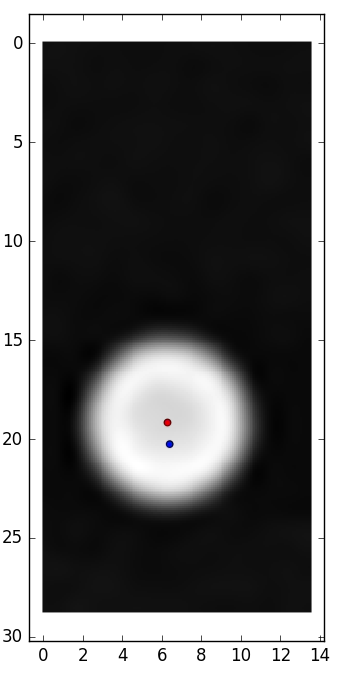
\includegraphics[scale=0.55]{python/ph2/centroid/CT_x100@0_centroids.png}
    \caption{CT @ 0}
    \label{fig:CT_x100_centroids@0}
  \end{subfigure}
  \begin{subfigure}[b]{0.32\textwidth}
    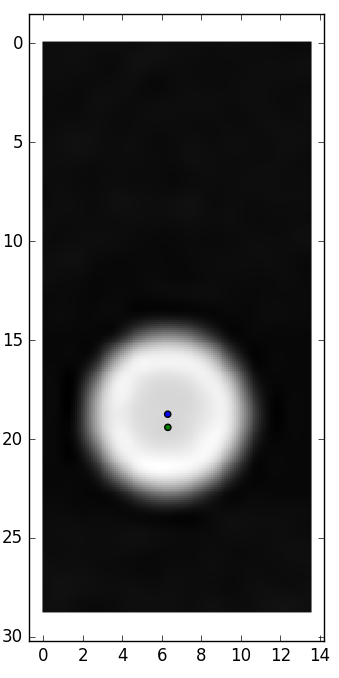
\includegraphics[scale=0.55]{python/ph2/centroid/CT_x100@150_centroids.png}
    \caption{CT @ 150}
    \label{fig:CT_x100_centroids@150}
  \end{subfigure}
  \begin{subfigure}[b]{0.32\textwidth}
    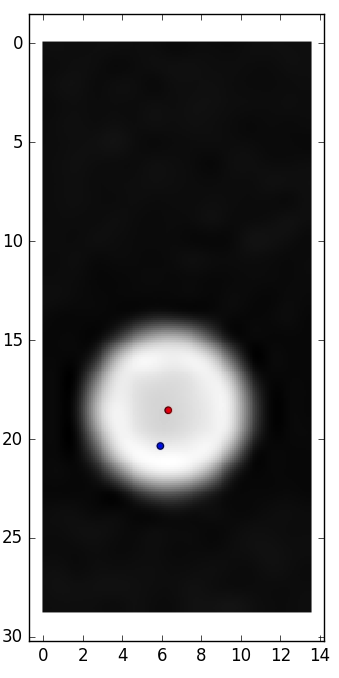
\includegraphics[scale=0.55]{python/ph2/centroid/CT_x100@304_centroids.png}
    \caption{CT @ 304}
    \label{fig:CT_x100_centroids@304}
  \end{subfigure}
  \begin{subfigure}[b]{0.32\textwidth}
    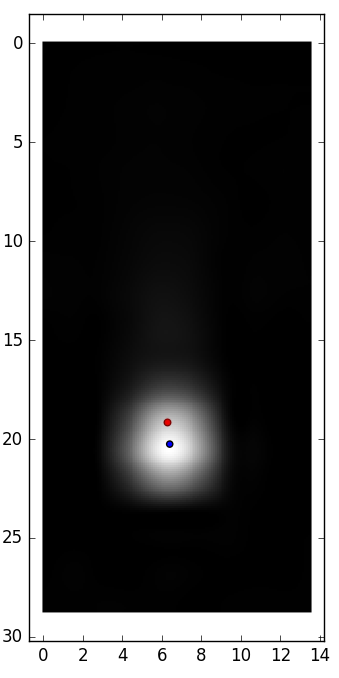
\includegraphics[scale=0.55]{python/ph2/centroid/MR_x100@0_centroids.png}
    \caption{MRI @ 0}
    \label{fig:MR_x100_centroids@0}
  \end{subfigure}
  \begin{subfigure}[b]{0.32\textwidth}
    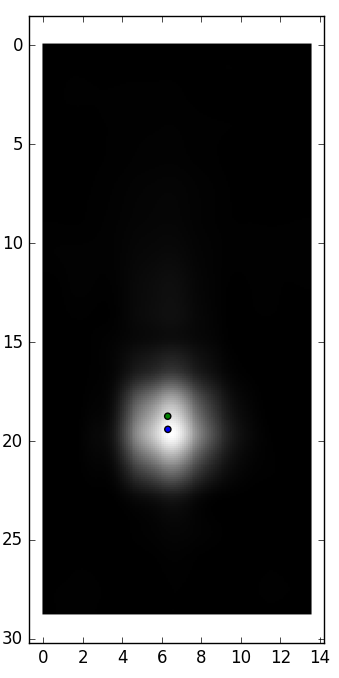
\includegraphics[scale=0.55]{python/ph2/centroid/MR_x100@150_centroids.png}
    \caption{MRI @ 150}
    \label{fig:MR_x100_centroids@150}
  \end{subfigure}
  \begin{subfigure}[b]{0.32\textwidth}
    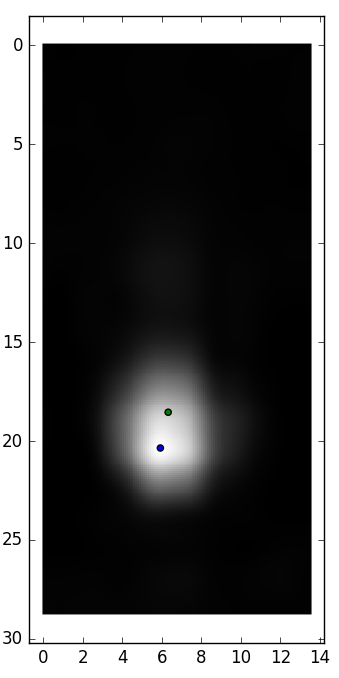
\includegraphics[scale=0.55]{python/ph2/centroid/MR_x100@304_centroids.png}
    \caption{MRI @ 304}
    \label{fig:MR_x100_centroids@304}
  \end{subfigure}
  \caption{MRI x100; blue dot centroid MRI, green dot centroid CT (same scale);\\ slice 150 is approximately at the isocentre, 0 on the very end of the image, 304 close to an air bubble}
  \label{fig:MR_x100_centroids}
\end{figure}

\clearpage

\subsection{DC}

\begin{figure}[!bp]
  \centering
  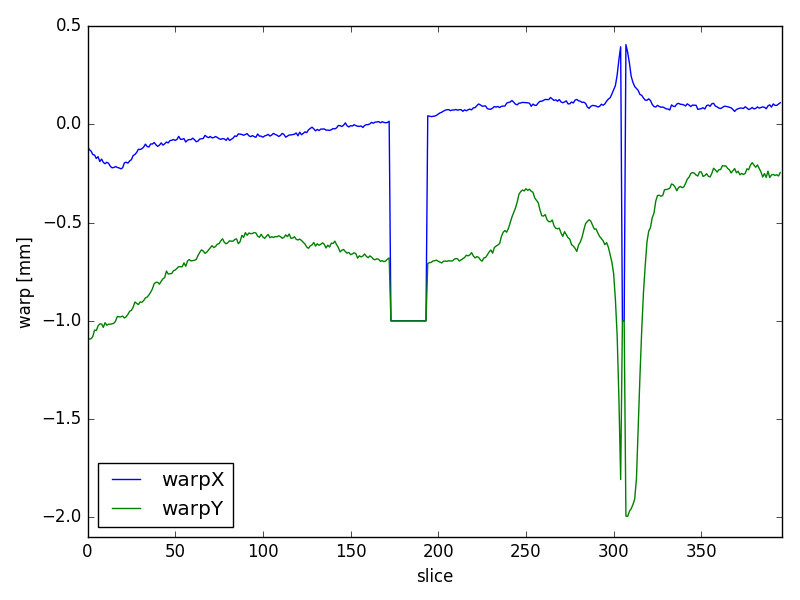
\includegraphics[scale=0.6]{python/ph2/warp/warpXY_x100--.png}
  \caption{warp XY [$mm$], CT-MRI x100}
  \label{fig:warpXY_x100}
\end{figure}

\begin{figure}[!tp]
    \centering
    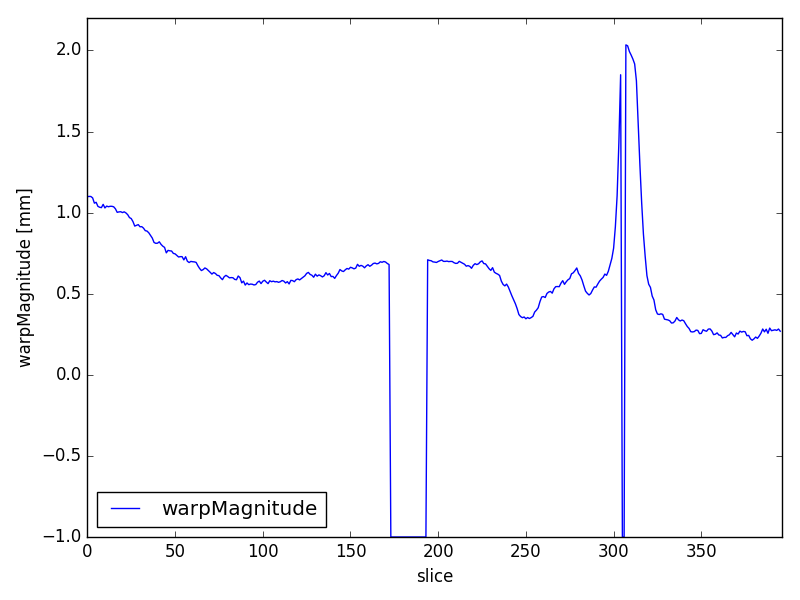
\includegraphics[scale=0.6]{python/ph2/warp/warpMagnitude_x100--.png}
    \caption{warp Magnitude [$mm$], CT-MRI x100}
    \label{fig:warpMagnitude_x100}
\end{figure}
\begin{figure}[!bp]
    \centering
    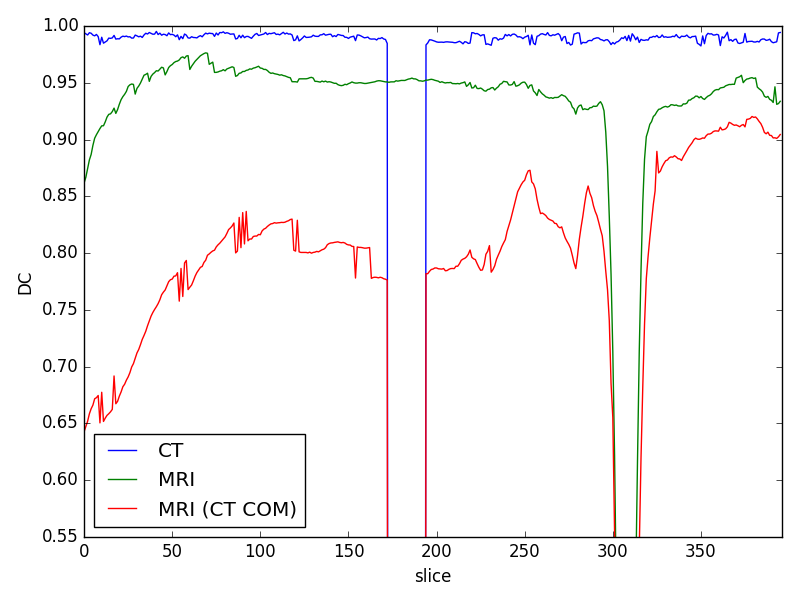
\includegraphics[scale=0.6]{python/ph2/dice/CT_MR_x100_DC.png}
    \caption{DC (optimised) for CT \& MRI \& MRI (using CT COM)}
    \label{fig:CT_MR_x100_DC}
\end{figure}

\begin{figure}[!tp]
    \centering
    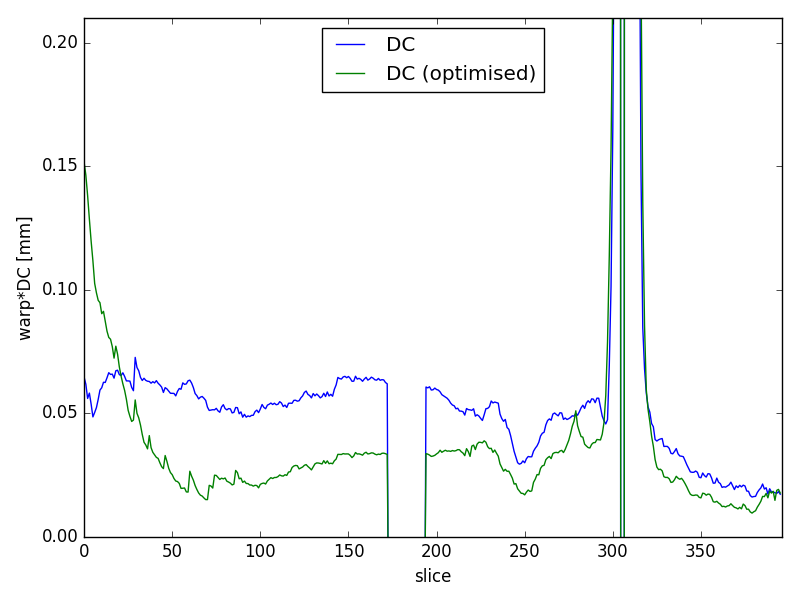
\includegraphics[scale=0.6]{python/ph2/warpDC/warpDC_x100.png}
    \caption{artificial indicator warp*DC using real DC and optimised DC of MRI x100}
    \label{fig:warpDC_x100}
\end{figure}
\begin{figure}[!bp]
  \centering
  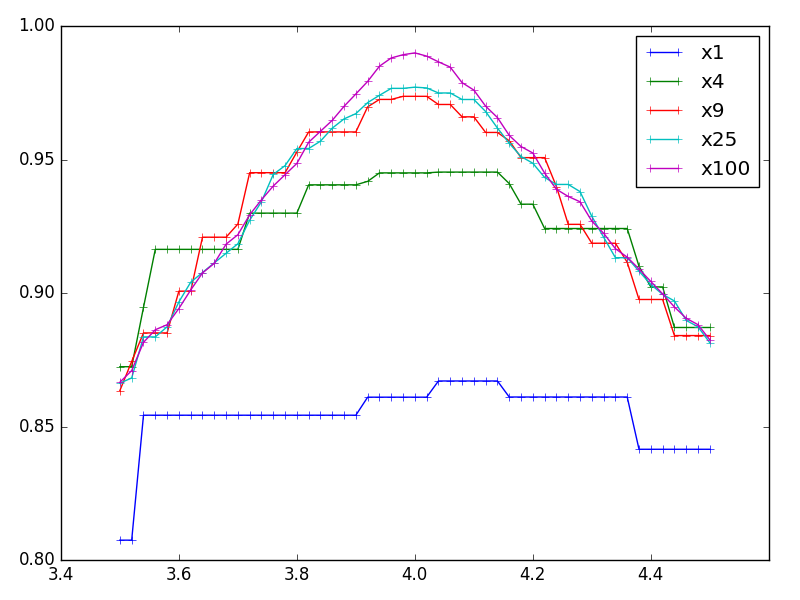
\includegraphics[scale=0.6]{python/ph2/dice/CT-51iter.png}
  \caption{CT: DC of varied radii \& resolutions}
  \label{fig:CT_dc}
\end{figure}

\begin{figure}[!tbp]
  \begin{subfigure}[b]{\textwidth}
    \centering
    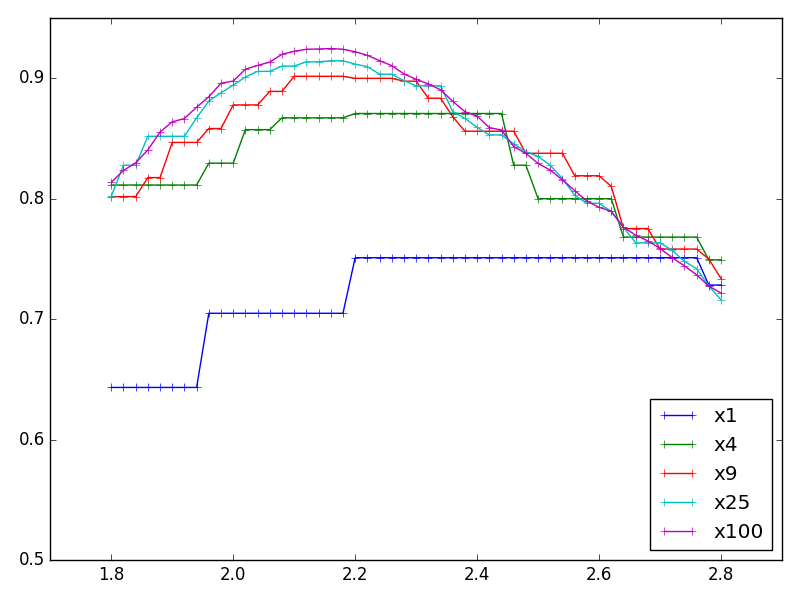
\includegraphics[scale=0.6]{python/ph2/dice/MR-51iter.png}
    \caption{MRI: DC of varied radii \& resolutions}
    \label{fig:MR_dc-opti}
  \end{subfigure}
  \begin{subfigure}[!b]{\textwidth}
    \centering
    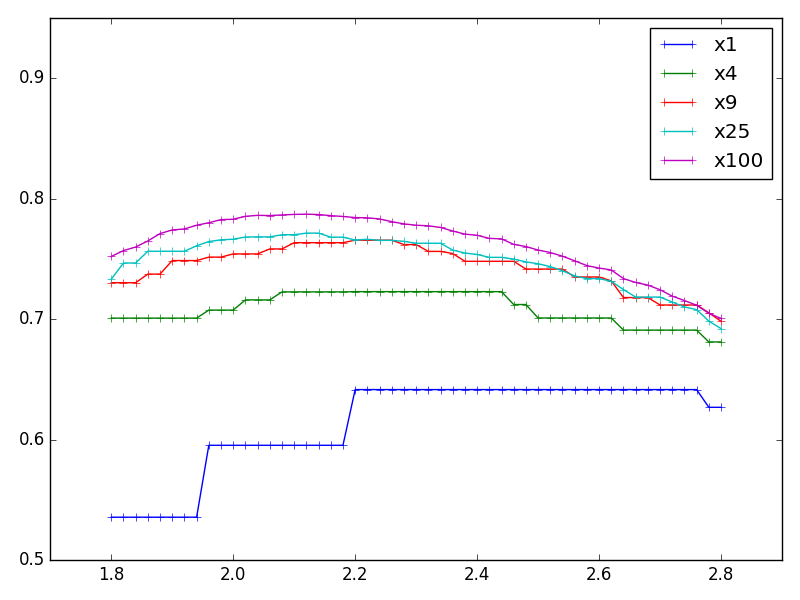
\includegraphics[scale=0.6]{python/ph2/dice/MR_CT-COM_51iter.png}
    \caption{MRI: DC of varied radii \& resolutions (using CT-COM)}
    \label{fig:MR_CT-COM_dc-opti}
  \end{subfigure}
  \caption{}
  \label{fig:MR_dc}
\end{figure}


The obtained dice coefficient varies not only because of the circle's centre and the radius, it also depends on the images resolution.
Figure \ref{fig:CT_dc} and \ref{fig:MR_dc} show the DC (optimised) obtained using CT and MRI scans over resample rate.

\todo{include table with actual RESULTS that are spit out by script and reference to python code (which will be in appendix)}
\todo{PIOTR: create colour coded images}

% \begin{figure}[!tbp]
%   \begin{subfigure}[b]{\textwidth}
%     \centering
%     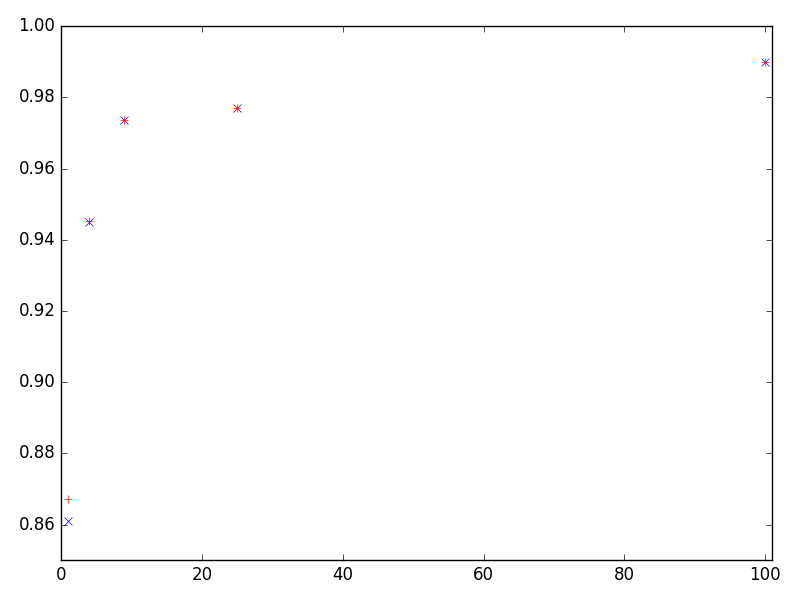
\includegraphics[scale=0.65]{python/ph2/dice/CT_dice-comparison_fast-51iter.png}
%     \caption{CT: x1, x4, x9, x16, x25, x100}
%     \label{fig:MR_dice-comp}
%   \end{subfigure}
%   \begin{subfigure}[b]{\textwidth}
%     \centering
%     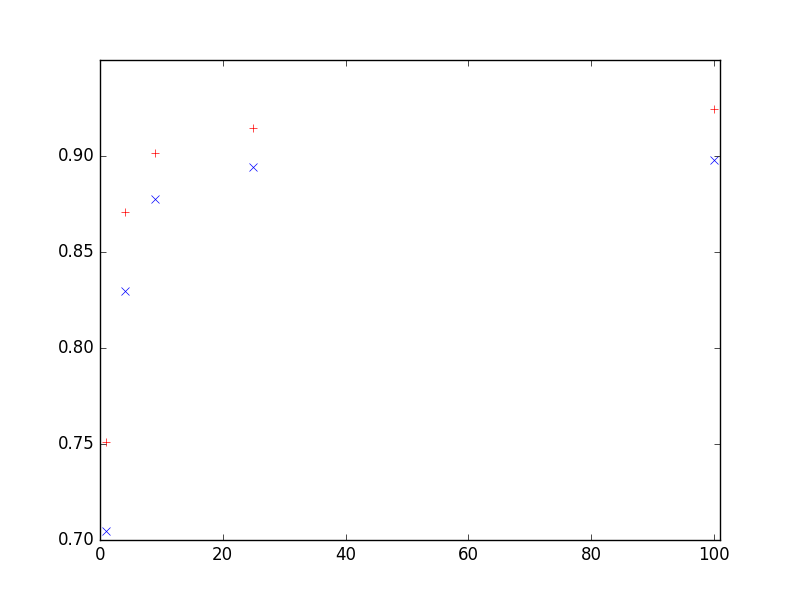
\includegraphics[scale=0.65]{python/ph2/dice/MR_dice-comparison_fast-51iter.png}
%     \caption{MRI: x1, x4, x9, x16, x25, x100}
%     \label{fig:MR_dice_comp}
%   \end{subfigure}
%   \caption{}
%   \label{fig:dice_com}
% \end{figure}

% image of COM shift
%This kind of comments need to go to the dicussion. As mentioned above here you report on the results. So the numbers, tables and images. You can write the the rod X was better vissible than Y. One iquid waseasier to fill than other. But what you thing is more useful and why (considering all pros and cons) you need to put in the dicussion. That is why it is called discussion :)



\chapter{Discussion}
% o Interpretation of results, putting them in context with literature
% o Discuss only results which were presented in the results section and do not repeat them one by one
% o Which impacts have your results on the scientific community?
% o provide an assessment of the weaknesses and strengths of your work
% o At least 5 pages

\section{Phantom design}

To be able to assess the spacial distortion of an MRI scan, a rigid object with known dimensions needs to be scanned so the cross referencing to the ground truth can be performed.
Such phantoms are commercially available, but often expensive and designed for a specific calibration protocol.
Some institutions build their own to fulfil exactly the requirements of a given application.
The scanner used at the AKH is a relatively rare model, which is why no off-the-shelf phantom that would fit its coil is available.

A previously used phantom did not fill the whole FOV, while at the same time weighing about 45kg.
This was due to the fact that it resembled a cuboid water tank with a thin plastic rod construction inside.
As the peripheral zones of the FOV are those where distortion is most pronounced, a bigger phantom was needed to assess those regions.
The new design deals reaches the outer regions and weighs much less at the same time.\\

Due to the underlying physics, plastics are not visible in MR scans, but CT scans visualize them. 
See figure \ref{fig:sagittal_comparison} for a comparison (MRI/CT visibility).
Therefore, it was decided to use plastic rods with a suitable fluid filling.
Such a liquid should be easily produced, non-toxic and yielding sufficient signal in MRI scans.

Commercially available phantoms often resemble water filled tanks containing plastic grids as a reference.
This design results in stronger signal, but exceeds practical weight.
There are few brands offering solutions utilising liquid fiducial markers in the shape of pellets.
They are arranged in a regular pattern surrounded by air or plastic.
The AKH's design however relies on replaceable rods, which makes it a novelty.

\subsection{Observed issues}

Interestingly, all water based solutions seemed to have evaporated partly.
As the rod filled with liquid \textbf{\#15} has dried starting at the end with the plastic stopper, it seems likely that, at least in this particular case, the plastic stopper did not effectively close the rod.
It might also be that the rod itself does not prevent volatile liquids from escaping slowly.
This was tested in a small experiment where an empty, closed rod was placed underwater.
After some time, water bubbles formed along its wall.
An airtight container might have led to other conclusions regarding the formation of air bubbles.
It is hard to tell if they were caused by evaporation only or if dissolved gases played a role, too.
Whatever the reasons are, the use of water based liquids seems to be suboptimal.
Despite this, the observed behaviour will still be discussed as a future airtight phantom design might benefit from drawn conclusions.

\section{Tested solutions}

For measuring the position of the rods in the CT scans, the plastic rods without filling would be enough already.
That is why the visibility of the liquids on CT is not important at all.
Hollow plastic rods would not be visible on the MRI scans, though.
From now on 'signal (strength)' or 'visibility' will refer to MRI scans only (see table \ref{tab:visibility}).

\subsection{Thoughts about choosing possible candidates}

The tested solutions were chosen for a number of reasons:
\begin{itemize}
\item Generally, imaging techniques aims for a high signal-to-noise ratio. Therefore, Liquids resulting in brighter pixels are favoured.
\item The amount of gas in the rods should be minimised.
\item If air bubbles form, tilting the entire phantom slightly should be enough to move them to one side. The FOV of the MRI scanner is too small to show the entire phantom anyway.
\item Most tested fluids are based on water, because this makes them easy to empty and clean.
They could then be filled again with a different liquid if needed.
\item Preferably, the components which are chosen to be used for the entire phantom should be non-toxic.
\end{itemize}

\vspace{1cm}

Rod \textbf{\#1} was filled with plain distilled water and intended to be used only as a reference.
It was clear from the beginning that it would not result in high signal and was never considered a possible filling.

\subsubsection{Aiming for high SNR}
To achieve a better SNR, liquids \textbf{\#2} to \textbf{\#10} and \textbf{\#14} to \textbf{\#15} are based on a solution of sodium chloride ($NaCl$ concentration of $0.36 \, g/L$) and copper(II) sulfate pentahydrate ($CuSO_4\cdot5H_2O$ concentration of $1.96 \, g/L$ as suggested by AAPM MR Subcommittee \cite{Jackson2009};  \textbf{\#3} and \textbf{\#4} contain double and ten-fold the concentration) in distilled water.
Most of these liquids resulted in an about 5 times brighter signal than plain distilled water.
Regarding the toxicity of $CuSO_4\cdot5H_2O$, the minimum dose to have caused acute toxic effects in humans is reported to be $11 mg/Kg$.
%As the concentration of $CuSO_4\cdot5H_2O$ is only $1.96 \, g/L$, even a young patient of 4 years and $15kg$ would need to drink more than 80mL to reach that threshold.
%Also, ingestion usually leads to vomiting triggered by its irritating effect on the gastrointestinal tract, which would stop further (more severe) toxic effects from happening.
%Keeping the scanner bed clean and checking the phantom for leakage before and after use should be sufficient to prevent an intoxication.
% http://pmep.cce.cornell.edu/profiles/extoxnet/carbaryl-dicrotophos/copper-sulfate-ext.html

\vspace{1cm}

Primovist (\textbf{\#11} to \textbf{\#13}) is a common contrast agent used for MRI scans \cite{VanBeers2012, Rohrer, primovist} intended to yield an even stronger signal than $CuSO_4\cdot5H_2O$ based liquids.
The major drawback is its tendency to separate from the water and stick to the container's wall.
This results in low signal at the centre and high signal along the wall, which would not necessarily pose a problem, but as the liquid forms bubbles, it is not guaranteed that the walls would be covered homogeneously.
The uneven distribution might result in wrong calculations, especially if the software tool is not programmed to cope with this behaviour.
At the same time the removal would be hardly possible.

\subsubsection{Handling dissolved gas}
Unfortunately, dissolved gases may eventually leave the liquid and form air bubbles trapped in the rod.
To improve the mobility of trapped air bubbles, generic washing-up soap was added (\textbf{\#5}, \textbf{\#6}, and \textbf{\#7}; suggestion by Data Spectrum Corporation \cite{bubbles}).
%The smallest amount of 1 g/L was already enough to result in sufficient mobility and an even lower concentration might also be acceptable.
The higher concentrations of soap were tested as reference.
%Interestingly, the rod filled with this solution contained the least amount of gas after 2 months.
If the liquid should happen to leak from the rod, the relatively low concentration of soap would not add to its toxicity.
%The visibility recorded was among the higher candidates, too.
For those reasons, and because the liquid is cheap and easy to produce, it appears to be a promising candidate.

\vspace{1cm}

Liquids \textbf{\#8} ($0.36 g/L$), \textbf{\#9} ($3.6 g/L$) and \textbf{\#10} ($36 g/L$) contain ascorbic acid.
Adding this was supposed to reduce forming of air bubbles by binding dissolved oxygen and eventually degrade to dehydro-ascorbic acid and water.
The amount suggested by \cite{Abtahi2008, Bodannes1979} is $0.00204 \; mol/L$ which corresponds to approx. ($0.36 g/L$).

\vspace{1cm}

In an attempt to limit the forming of gas, \textit{agar} was used in solutions \textbf{\#14} and \textbf{\#15}.
Agar and agarose are commonly used as basic reference material for MRI phantoms \cite{BuccioliniCiraolo1989, Mathur-DeVre1985}
%Since the produced gel cannot be removed from the rods as easily as liquid candidates, and forming air bubbles were also not moving, agar is not suited for this phantom.

\subsubsection{Non water-based liquids}
As an alternative 2 oils were proposed.
Since oil is neither soluble in air, nor able to evaporate, a rod completely filled with oil should stay free from air bubbles.
Yet, oil is not as easily removed from a rod as a water based liquid.
At the same time, it might not be necessary to ever replace the oil.
Once filled, the rods could be used until the surrounding plastic breaks or starts leaking.
Using vegetable oil would be a non-toxic solution, but has been ruled out as a filling from the beginning, because it would eventually rot.
Mineral oil on the other hand does not rot, however, it might be toxic if consumed.
%As the generic motor (\textbf{\#16}) oil resulted in the highest signal intensity of all candidates it seems to be a good alternative to water based liquids.
%The silicon oil (\textbf{\#17}) on, the other side, had a low signal compared to most candidates and is therefore not suited.


\subsection{Choosing a promising candidate}
As all rods containing water continued to lose liquid due to evaporation, only the early forming of air bubbles might indicate whether solutions effectively hinder dissolved gases to result in trapped air bubbles.
Apart from the solutions containing ascorbic acid (\textbf{\#8} ($0.36 g/L$), \textbf{\#9} ($3.6 g/L$)) all water based liquids produced some air bubbles after at least two days (see table \ref{sec:sol-mech}).
Considering the low visibility of \textbf{\#9}, the only suitable water based liquid capable of staying free from air bubbles might be \textbf{\#8}.
At the same time, long-term observations performed in an airtight container might have shown that even \textbf{\#8} only delays the process.
In the case of the used rods, such a conclusion cannot be drawn with certainty.

The rod containing the highest concentration of ascorbic acid showed a yellow colouring, caused by dehydroascorbic acid which is the result of a oxygenation process.
However, as the high concentration in \textbf{\#9} and \textbf{\#10} led to a radical reduction in signal with the tested MRI sequence, this solutions is not considered a suitable filling anyway.

Primovist (\textbf{\#11} to \textbf{\#13}) lead to a good signal, but its limited mobility of air bubbles; its tendency to accumulate along the wall; and the difficulty of cleaning the rods rule it out as a candidate.

If the forming of  a small amount of gas is not considered a problem, adding soap appears to be a reasonable solution.
The smallest tested amount of soap (\textbf{\#5}, 1 g/L) was already enough to result in sufficient mobility of air bubbles, and an even lower concentration might also be acceptable.
Interestingly, the rod filled with this solution contained the least amount of gas after 2 months, but this might be because the particular rod closed better than the others.
The visibility recorded was among the higher candidates, too.
For those reasons, and because the liquid is cheap and easy to produce, it is a promising candidate.

Solutions containing \textit{agar} (\textbf{\#14} and \textbf{\#15}) are even harder to remove from rods if not impossible.
As they might lead to air bubbles, too, which cannot be moved to either side of the rod, agar is not suited for this phantom.

Finally, the synthetic motor oil (\textbf{\#16}) resulted in the highest signal intensity of all candidates.
Besides the question of its toxicity, it seems to be a good alternative to water based liquids.
The silicon oil (\textbf{\#17}) on, the other side, had a low signal compared to most candidates and is therefore not suited.


\section{Distortion}

\subsection{Calculation Methods}
\texttt{DC} and warp calculated with the simple and iteration method do not differ much.
Moreover, both methods choose very similar thresholds for their calculations (see header of appended '.txt' output file)
As the simple method uses additional information on the rod's true dimension, it is supposed to yield accurate, reliable results.
The iteration process, oblivious to the imaging modality, supports this claim as it produces very similar numbers.\\

The biggest difference in the results obtained with both methods are the values in the region of the air bubble in rod \#5:
Slices 303-310 in table \ref{tab:spit-out-5} mark the area where the maximum brightness dropped significantly due to the absence of liquid (see figure \ref{fig:ph2_MR_x100_brightness}).
The simple method for finding the COM did not manage to calculate coordinates in this region, due to the lack of pixels above the threshold based on the reference slice (which was ~827; see appendix).
Consequently, warp and DC for MRI were set to '-1'.
However, the iteration method tried various thresholds and settled for the one resulting in the highest average DC for the whole scan.
As slices with values of '-1' influence the average dramatically, the chosen threshold is low enough (~339; see appendix) to include some of the brightest pixels in slices 303-310.

\begin{figure}[!tbh]
\centering
	\begin{subfigure}[b]{0.32\textwidth}
		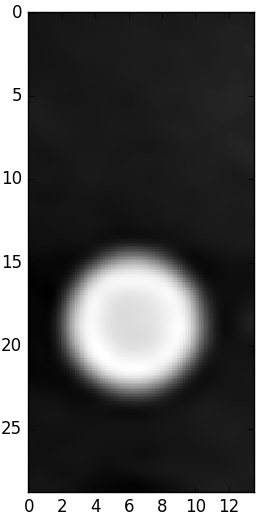
\includegraphics[width=\linewidth]{../fig/python/ph2/brightness/ph2_CT_pane@175}
		\caption{slice 175}
		\label{fig:ph2_CT_x100_pane_0}
	\end{subfigure}
	\begin{subfigure}[b]{0.32\textwidth}
	  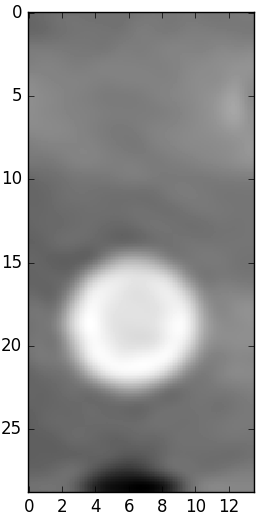
\includegraphics[width=\linewidth]{../fig/python/ph2/brightness/ph2_CT_pane@176}
	  \caption{slice 176}
	  \label{fig:ph2_CT_x100_pane_1}
	\end{subfigure}
	\begin{subfigure}[b]{0.32\textwidth}
	  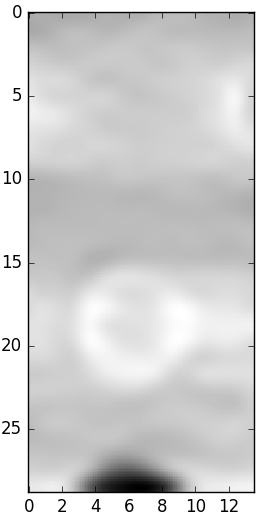
\includegraphics[width=\linewidth]{../fig/python/ph2/brightness/ph2_CT_pane@177}
	  \caption{slice 177}
	  \label{fig:ph2_CT_x100_pane_2}
	\end{subfigure}
  \caption{Slices at edge of plastic pane in CT image showing rod \#5 (true colours): a black crescent remains at the bottom where there is a hole in the pane that is not filled with a rod at the moment}
  \label{fig:ph2_CT_x100_pane}
\end{figure}

\subsection{Irregularities}
All obtained CT scans include a region where the plastic panes are visible.
Figure \ref{fig:ph2_CT_x100_pane} shows how the plastic pane makes it impossible to define the rod on the CT image.
These areas cannot be used for distortion assessment as the COM cannot be calculated reliably.
Figures \ref{fig:ph2_CT_x100_brightness} and \ref{fig:ph3_CT_x100_brightness} exhibit spikes in the average brightness where the image shows a plastic pane.
The script recognised this difference and marked all affected slices as 'irregular'.
Consequently, in table \ref{tab:spit-out-5} and \ref{tab:spit-out-16}, the values of the COM shift ($warp_x$, $warp_y$, $warpM$); the DC for CT using the CT-centroid ($DC_{CT}$); and the DC for MRI using the CT-centroid ($DC_{MR(CT-COM)}$) are all set to '-1'.

\subsection{Measured distortion - Rod \#5}

Figure \ref{fig:MR_x100_centroids} visualises the centroid shift at interesting slices of rod \#5.
It is clearly visible that the shift is bigger at the end of the rod (slice 0) compared to a slice close to its middle (slice 171).
The values of $warpM^*$ in table \ref{tab:spit-out-5} verify this (1.0623mm > 0.6926mm).
Furthermore, the distortion measured at the location of the air bubble (slice 304) shows a maximum for the COM shift ($warpM^*$ = 1.5748mm) and a minimum for the DC ($DC^*_{MR}$ = 0.6762).
These values originate not from true spatial distortion, but are caused by the presence of gas in the rod.
Since the bubble floated on top of the liquid, the COM shift is most pronounced in the y direction (up-down) as shown by figure \ref{fig:ph2_warpXY_x100}.
The overall impact on the area of 110mm to 140mm is clearly visible in figures \ref{fig:ph2_warpMagnitude_x100} and \ref{fig:ph2_DC_x100}.
In conclusion, it is imperative for the distortion assessment to exclude bubbles from the FOV.

\subsection{Measured distortion - Rod \#16}

Similar to the findings for rod \#5, the distortion is bigger in the peripheral regions of the FOV (see figure \ref{fig:ph3_DC_x100}).
Interestingly, the y shift changes its orientation around the centre (see figure \ref{fig:ph3_warpXY_x100}).
This might be a local feature of the distortion and cannot be put in relation, because no distortion map of the entire FOV is available yet.

As rod \#16 does not contain any air bubbles, the brightness plotted in figure \ref{fig:ph3_MR_x100_brightness} shows no sudden drops.
However, the left hand side has a drastically lower signal strength than the right.
A closer look revealed that rod \#16 contained oil of two different colours.
It seems that some residue of the other oil, which was injected into rod \#17, was still present in the syringe when rod \#16 was filled.
To avoid this, the injecting syringe and the capillary were flushed with the next liquid before injection.
This procedure was not enough to clean it thoroughly.
The liquids separated into parts with different density while the rod was stored upright and were still distributed unevenly during imaging.
To avoid this problem in the future, a new and unused syringe should be used for filling.\\

It is likely, that this will have influenced the calculated warp and DC as the lighter oil (which results in a different signal strenght) will have floated on top of the other resulting in an unwanted shift of the calculated COM.
This might explain why the y shift changes its orientation close to the iso centre as this is the point where the signal intensity starts to change, too.
To be sure of the actual impact of the oil mix on the distortion assessment, a new rod should be filled and the imaging repeated.
For now, the already gained results will be used as no new measurement could be obtained in the limited time that the scanner is available for such experiments.


In the region beyond -330, there is a drop of the DC for the CT.
Investigations revealed that this is caused by sticky tape attached to the rod to hold it in place during transport from the CT scanner to the MRI scanner.
The values calculated for this area are most likely influenced by this.


\subsection{Effect of resampling}


Figures \ref{fig:ph2_warpMagnitude_x1-100} and \ref{fig:ph3_v2_warpMagnitude_x1-100} depict the measured $warpM^*$ of rod \#5 and \#16 for x1 and x100 resample rates.
The location shift calculated with x1 and x100 resample rate are relatively close (see tables \ref{tab:Delta-resample_5} and \ref{tab:Delta-resample_16}).\\

The calculated DCs for the scans in original CT resolution (x1) are shown in figures \ref{fig:ph2_DC_x1} and \ref{fig:ph3_DC_x1} and for a x4 finer resolution in figures \ref{fig:ph2_DC_x4} and \ref{fig:ph3_DC_x4}.
Compared to the DCs of the x100 resampled scans (figures \ref{fig:ph2_DC_x100} and \ref{fig:ph3_DC_x100}), the low resolution x1 yields significantly less smooth curves.
A resample rate of x4, on the other hand, is already much closer to the quality of the x100 scans.\\

While the original resolution might be sufficient for the calculation of the COM shift, the DC calculation benefits a lot from a interpolated image.
It is easier to spot significant changes as the plot shows less jumps.
At the same time, the computing time for calculations scales with the resolution of the images and should be kept minimal, because a future assessment would include more than 300 individual rods.

\subsubsection{Rod \#5}

\todo{interpret table \ref{tab:Delta-resample_5}}

\begin{table}[!tbh]
\centering
\begin{tabular}{l|rr}
                    & E         & $\sigma$   \\ \hline
$\Delta warpM^*$ [mm]  & 0.038     & 0.058    \\
$\Delta DC^*_{CT}$         & 0.002245  & 0.006838 \\
$\Delta DC^*_{MR}$         & 0.000518  & 0.019070 \\
$\Delta DC^*_{MR(CT-COM)}$ & -0.008905 & 0.022050
\end{tabular}
\caption{Change in calculated distortion due to resample rate; rod \#5; x1 compared to x100}
\label{tab:Delta-resample_5}
\end{table}

\begin{figure}[!tbh]
    \centering
    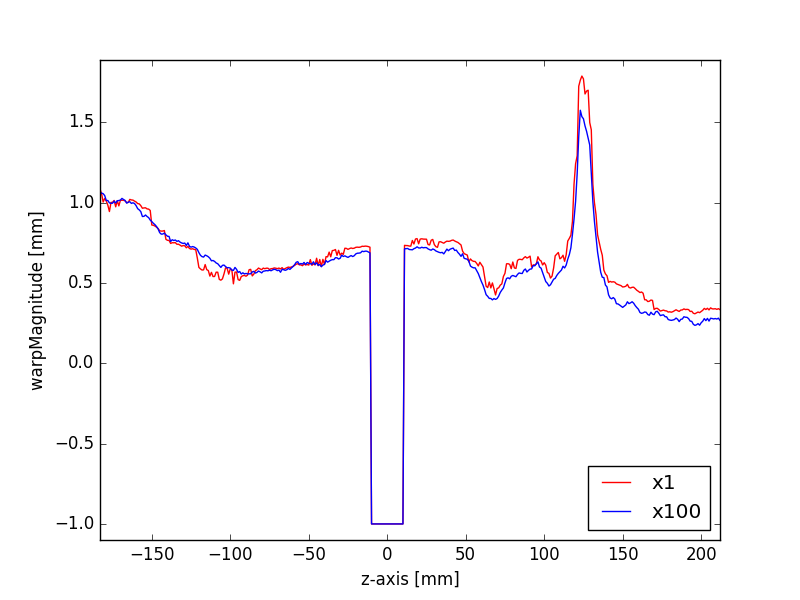
\includegraphics[scale=0.6]{../fig/python/ph2/warp/warpMagnitude_x1-100_iter.png}
    \caption{Rod \#5: warp Magnitude [$mm$] (iteration method), CT-MRI x1 and x100}
    \label{fig:ph2_warpMagnitude_x1-100}
\end{figure}

\begin{figure}[!bth]
    \centering
    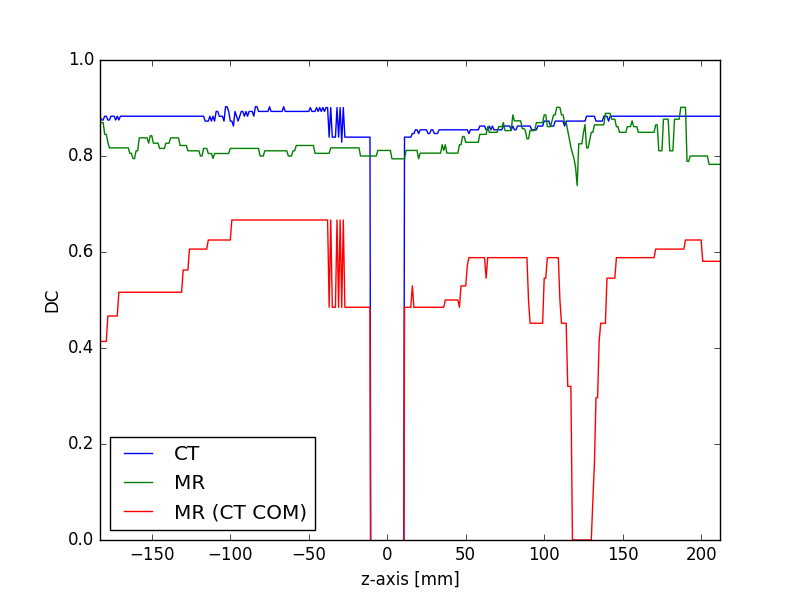
\includegraphics[scale=0.6]{../fig/python/ph2/dice/ph2_DC_x1_iter.png}
    \caption{Rod \#5: DC (iteration method) for CT \& MRI \& MRI (using CT COM); x1}
    \label{fig:ph2_DC_x1}
\end{figure}

\begin{figure}[!bth]
    \centering
    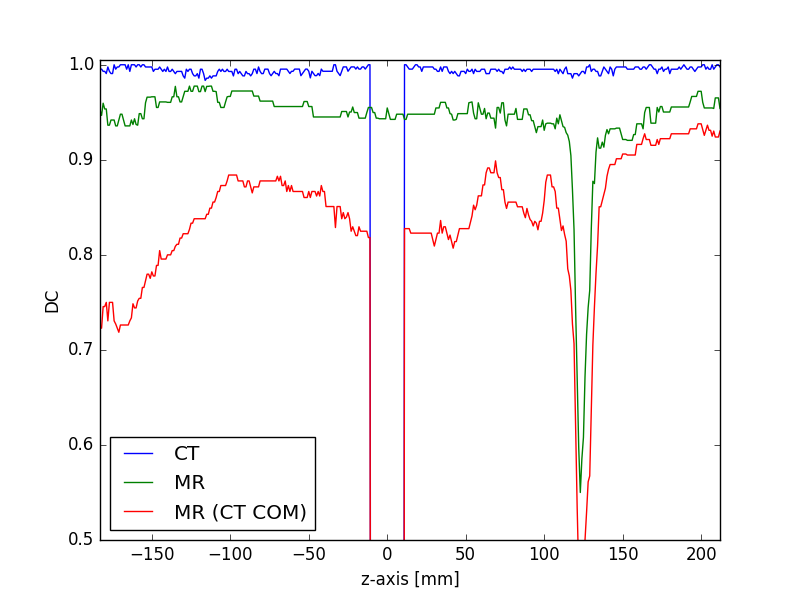
\includegraphics[scale=0.6]{../fig/python/ph2/dice/ph2_DC_x4_iter.png}
    \caption{Rod \#5: DC (iteration method) for CT \& MRI \& MRI (using CT COM); x4}
    \label{fig:ph2_DC_x4}
\end{figure}

\clearpage

\subsubsection{Rod \#16}

\todo{interpret table \ref{tab:Delta-resample_16}}

\begin{table}[!tbh]
\centering
\begin{tabular}{l|rr}
                    & E         & $\sigma$   \\ \hline
$\Delta warpM^*$ [mm]  & 0.005     & 0.025    \\
$\Delta DC^*_{CT}$         & -0.001849  & 0.007117 \\
$\Delta DC^*_{MR}$         & 0.004835   & 0.019823  \\
$\Delta DC^*_{MR(CT-COM)}$ & 0.012554   & 0.019429
\end{tabular}
\caption{Change in calculated distortion due to resample rate; rod \#16}
\label{tab:Delta-resample_16}
\end{table}

\begin{figure}[!tbh]
    \centering
    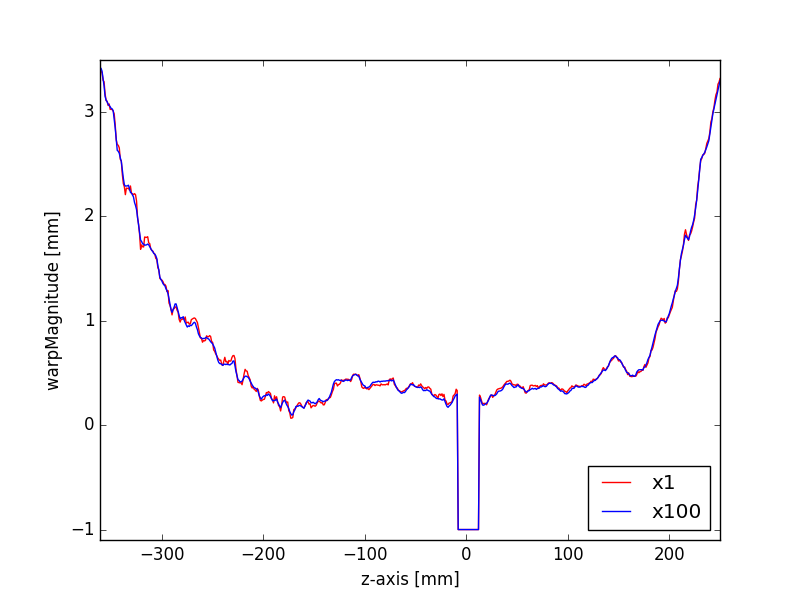
\includegraphics[scale=0.6]{../fig/python/ph3_v2/warp/ph3_MR_v2_x1-100_warpMagnitude_iter.png}
    \caption{Rod \#16: warp Magnitude [$mm$] (iteration method), CT-MRI x1 and x100}
    \label{fig:ph3_v2_warpMagnitude_x1-100}
\end{figure}


\begin{figure}[!tbh]
    \centering
    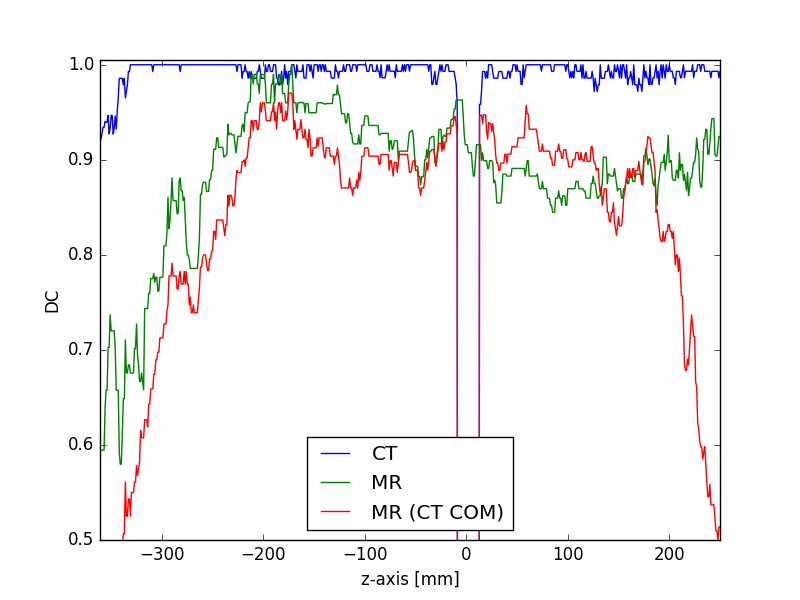
\includegraphics[scale=0.6]{../fig/python/ph3_v2/dice/ph3_MR_v2_x1_DC_iter.png}
    \caption{Rod \#16: DC (iteration method) for CT \& MRI \& MRI (using CT COM); x1}
    \label{fig:ph3_DC_x1}
\end{figure}

\begin{figure}[!tbh]
    \centering
    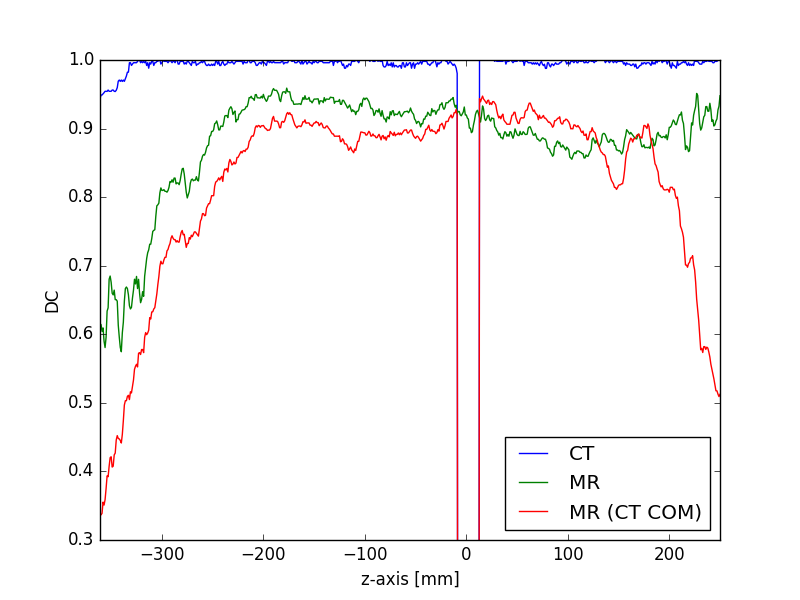
\includegraphics[scale=0.6]{../fig/python/ph3_v2/dice/ph3_MR_v2_x4_DC_iter.png}
    \caption{Rod \#16: DC (iteration method) for CT \& MRI \& MRI (using CT COM); x4}
    \label{fig:ph3_DC_x4}
\end{figure}

%\todo{discuss what is visible on the graphs in results section}
%\todo{interpret data table spit out by script}
%\todo{scale of distortion, bigger on the sides as expected}
%\todo{only x,y direction. future design needs objects going from left to right, too.}

\chapter{Conclusion and Outlook}
% o Summary of study
%  Most important results and their meaning/impact and conclusions
%  Outlook
%  open questions
%  Next steps
\section{Filling for phantom}

As topping up over 300 rods regularly is too time consuming, and all water-based liquids continued to evaporate, they are not long-term solution for this phantom.
They are, however, useful for prototyping.
For short time experiments with this phantom (not airtight rods) \textbf{\#5} is recommended, because the soap allows the air to be moved out of the FOV.
If another set of rods with airtight walls were obtained, adding ascorbic acid to the solution (a combination of \textbf{\#5} and \textbf{\#8}) might be an even better filling:
\begin{itemize}
\item  distilled water
\item  $0.36 \, g/L$ of $NaCl$
\item  $1.96 \, g/L$ of $CuSO_4\cdot5H_2O$
\item  $1 \, g/L$ of soap
\item  $0.36 g/L$ of ascorbic acid
\end{itemize}
In that case, the forming of air bubbles might be either avoided entirely (due to the ascorbic acid) or delayed and then easily taken care of by tilting the whole phantom slightly to move the bubbles out of the FOV.
The long-term behaviour of the mix might lead to adverse properties and should be tested, though.

In the current set-up, it seems best to fill the rods of the phantom with the type of oil that does not rot and yields high signal.
The tested synthetic motor oil (\textbf{\#16}) fits those requirements.

\section{Recommended resample rates}

The accuracy of the distortion assessment, especially of the DC calculation, can be enhanced by using interpolated scans.
Resample rates of x4, x9, x25 and x100 were used to create finer images which were all analysed using the same algorithms.
The original resolution (x1) might be sufficient for the COM shift calculation, but the DC curve gains significant smoothness at already x4 finer resolution.
This small interpolation could be already enough to increase accuracy while keeping necessary computing power low.
A future distortion assessment of the whole FOV with 300 individual rods would profit from a effective procedure at low resolution.
Using the simple method to find the COM would use less time, too.

    
\section{Future improvement of software tool}

The developed tool took a simplified approach to the problem by looking only at a single rod.
Distortion assessment can be performed using the generated tool, however, it needs to be implemented on more general scale to be able to measure the distortion for all the rods automatically.
This could be done by a auto-trace function which detects individual rods and applies the already implemented algorithms to each of them separately.\\

The two implemented methods of finding COM and DC need to be assessed themselves.
In order to tell which of the two gets closer to the absolute truth, additional checks should be performed.
A possible accuracy test could look like this:
two CT scans of the phantom which differ only by a known displacement of one rod are registered and resampled.
The software tool is used to calculate the COM shift between the images which can be compared to the real displacement.\\

At the moment the iteration method does not take into account the steepness of the DC curve.
In some cases this might result in neglecting the left hand side close to very low percentages.
This happens when the maximum lies roughly in the middle of the current range, but a little bit to the left.
Because the slope is steeper on the left (close to 0\%), a value representing the left hand side (also close to 0\%) yields a much lower result than the value on the right hand side (flat slope).
This should be taken into account during further improvement of the method.\\

In the current version of the software tool, only changes in the mean brightness are used to characterise irregularities.
It might be usefull to consider drops in the peak brightness as irregularities, too.
This way, the distortion would not be calculated in the region of an air bubble.
For the time being, running the script over those regions might aid troubleshooting and give better understanding how to improve the code.\\

%In cases where the COM cannot be calculated, it could be interpolated using neighbouring slices.

\section{Scale of distortion}

For the investigated position of the rod (rod \#16), the obtained values for the occurring spatial distortion report a COM shift below $1mm$ in a region of at least $40cm$ (from -283mm to 185mm; simple method).
This does not rule out the possibility of using the MR scanner for radiotherapy planning.
Whether the distortion is small enough to guarantee accurate treatment planning can only be discussed after a map for the entire FOV has been created.

\cleardoublepage
%\pagenumbering{roman} \setcounter{page}{1}
%\nocite{*}
\printbibliography
%\input{thanks.tex}

\chapter*{Appendix}
\addcontentsline{toc}{chapter}{Appendix}

The current version of the python script 'FunITK.py' with all functions described in this thesis used to calculate the presented numbers is available at:\\
\url{https://github.com/cyberspeck/mri-for-rt/blob/master/scripts}

The data of the cropped images showing rod \#5 and \#16, the created '.txt' and '.mha' files are stored at: \\ \url{https://github.com/cyberspeck/mri-for-rt/tree/master/data} \\

The following pages contain today's version of the python script 'FunITK.py' and the generated data for rod \#5 \& \#16.
\includepdf[pages=-]{pdfs/FunITK.pdf}
\includepdf[pages=-]{pdfs/rod_5.pdf}
\includepdf[pages=-]{pdfs/rod_16.pdf}

\end{document}